\documentclass[12pt,a4paper]{article}
\usepackage[utf8]{inputenc}
\usepackage{amsmath}
\usepackage{amsfonts}
\usepackage{amssymb}
\usepackage{graphicx}
\usepackage{tabularx}
\usepackage{ltablex}
\usepackage[export]{adjustbox}
\usepackage{caption}
\usepackage{float}
\usepackage{fancyhdr}


\author{Guillaume Quint \& Francesco Bonciani}
\title{Relazione Progetto di Base Dati 2019}
\pagestyle{fancy}

\begin{document}
\captionsetup[figure]{labelfont={it}, labelformat={default}, name={Figura }, font={footnotesize}}
\maketitle
\thispagestyle{empty}
\clearpage
\pagenumbering{Roman}
\renewcommand{\abstractname}{Visione d'insieme}


\begin{abstract}
L'obiettivo del progetto è la creazione di un database relazionale per la gestione di una catena di agriturismi chiamata \textit{FarmHouse 4.0}. 
Il database è conforme alle specifiche dell' industria intelligente \textit{Industry 4.0} e comprende diverse funzionalità di \textit{Data Analytics} implementate sul lato \textit{back-end}. 
Il database si occupa per ogni agriturismo della gestione delle stalle e degli animali che vi abitano.

Le stalle sono popolate da sensori che forniscono al database informazioni sullo stato di salute degli animali e sulle condizioni ambientali e di alimentazione che si registrano in ogni locale.
Viene anche tenuta traccia della posizione GPS degli animali che consente agli agriturismi di organizzare al meglio le aree di pascolo ed i loro allestimenti.
Ogni agriturismo effettua riproduzioni finalizzate ad ottenere specie sempre più resistenti e caratterizzate da un'elevata qualità del prodotto. Per ogni riproduzione si tiene traccia degli insuccessi e dei successi, compilando dipendente dal caso una scheda medica oppure una scheda di gestazione.
Entrambe vengono compilate da un'equipe di veterinari i cui dati vengono memorizzati anch'essi nel database.
Ogni animale deve sottoporsi a numerose visite che possono comparire nel database anche se non ancora effettuate, attraverso le quali i veterinari monitorano lo stato di salute degli animali e nel caso di malattia prescrivono terapie adeguate, con precise indicazioni sui farmaci utilizzati.
Le mungiture effettuate producono diversi tipi di latte organizzati in silos per garantire una composizione uniforme al prodotto, ed un gusto privo di contaminazioni; per lo stesso scopo vengono seguite ricette divise in fasi che vengono monitorate per effettuare un controllo della qualità della produzione.
Ogni prodotto appartiene a specifici lotti stoccati su scaffali all'interno di cantine o magazzini dipendentemente dalla necessità di stagionatura.
I clienti (registrati e non) possono prenotare degli alloggi all'interno di ogni agriturismo con i loro servizi aggiuntivi e/o effettuare escursioni guidate in varie aree delle tenute.
I clienti registrati possono acquistare i prodotti caseari e dispongono di un sistema di consegne e resi che tiene traccia delle tappe delle varie spedizioni.
Ogni cliente può inoltre recensire i prodotti relativi ai propri ordini, garantendo così un feedback utile al miglioramento dei processi produttivi.
In accordo alle specifiche di progetto fornite, si è scelto di schematizzare la base dati in cinque aree tematiche:
\begin{itemize}
\item Area Allevamento
\item Area Healthcare
\item Area Produzione
\item Area Soggiorno
\item Area Store
\end{itemize}
\end{abstract}
\pagebreak
\tableofcontents
\pagebreak

\pagenumbering{arabic}
\section{Glossario}
Sono qui descritte le varie entità e relazioni di ogni area, assieme ai relativi attributi e collegamenti con le altre parti del database.

Questo glossario è stato realizzato prima della progettazione del diagramma Entità-Relazioni: ogni modifica dovuta al processo di ristrutturazione verrà indicata nella relativa sezione \ref{sec:ristrutturazione} a pag. \pageref{sec:ristrutturazione}, oppure, nel caso di ridondanze tra entità e relazioni, anche nel paragrafo \ref{subsec:ridondanze-ent-rel} a pag. \pageref{subsec:ridondanze-ent-rel}
\subsection{Area Allevamento}
\subsubsection{Entità}
\label{Allevamento Entita}

\begin{center}

\setlength{\extrarowheight}{1.5pt}

\begin{longtable}{|p{0.14\linewidth}|p{0.20\linewidth}|p{0.36\linewidth}|p{0.20\linewidth}|}
\hline 
\textbf{Nome entità} 	& \textbf{Descrizione} & \textbf{Attributi} & \textbf{Collegamenti}\\ 

    
\hline
Abbevera\-toio 		& \begin{flushleft}\vspace{-15pt} Dispositivo per la distribuzione dell'acqua agli animali nei locali \end{flushleft}
					& \begin{itemize}
						\setlength{\itemindent}{-1em}
						\vspace{-25pt}
						\setlength\itemsep{-0.25em}
						\item acquaRestante
						
					\end{itemize}
					& \begin{flushleft}\vspace{-25pt} Locale, Pasto per Locale \end{flushleft}\\

\hline
Acqua 				& \begin{flushleft}\vspace{-25pt} Acqua eventualmente arricchita per l'idratazione degli animali \end{flushleft}
					& \begin{itemize}
						\setlength{\itemindent}{-1em}
						\vspace{-25pt}
						\setlength\itemsep{-0.25em}
						\item codiceAcqua
					\end{itemize}
					& \begin{flushleft}\vspace{-25pt} Pasto \end{flushleft}\\

\hline
Agrituri\-smo 			& \begin{flushleft}\vspace{-25pt} Struttura attrezzata per l'allevamento degli animali e l'accoglienza dei clienti conforme agli standard di \textit{Industry 4.0}  \end{flushleft}
					& \begin{itemize}
						\setlength{\itemindent}{-1em}
						\vspace{-25pt}
						\setlength\itemsep{-0.25em}
						\item nome
					\end{itemize}
					& \begin{flushleft}\vspace{-25pt} Cliente, Stanza, Stalla, Formaggio \end{flushleft} \\

\hline
Allestimen\-to 		& \begin{flushleft}\vspace{-25pt} Mangiatoie, Abbeveratoi, e dispositivi di illuminazione e condizionamento aria di ogni locale \end{flushleft}
					& \begin{itemize}
						\setlength{\itemindent}{-1em}
						\vspace{-25pt}
						\setlength\itemsep{-0.25em}
						\item codice
						
					\end{itemize}
					& \begin{flushleft}\vspace{-25pt} Locale \end{flushleft}\\

\hline
Ambientali 			& \begin{flushleft}\vspace{-25pt} Sensore di temperatura ed umidità del locale  \end{flushleft}
					& \begin{itemize}
						\setlength{\itemindent}{-1em}
						\vspace{-25pt}
						\setlength\itemsep{-0.25em}
						\item temperatura
						\item umidità
					\end{itemize}
					& \begin{flushleft}\vspace{-25pt} Locale \end{flushleft}\\

\hline
Animale 				& \begin{flushleft}\vspace{-25pt} Anagrafica degli animali di \textit{FarmHouse 4.0} \end{flushleft}
					& \begin{itemize}
						\setlength{\itemindent}{-1em}
						\vspace{-25pt}
						\setlength\itemsep{-0.25em}
						\item codice
						\item dataNascita
						\item peso
						\item altezza
						\item razza
						\item sesso
						\item specie
						\item famiglia
						
					\end{itemize}
					& \begin{flushleft}\vspace{-25pt} Mungitura, Latte, Scheda Medica, Animale Acquisito, Terapia, GPS, Indici Salute, Riproduzione \end{flushleft}\\ 

\hline
Animale Acquisito 	& \begin{flushleft}\vspace{-25pt}Generalizzazio\-ne di Animale \end{flushleft}
					& \begin{itemize}
						\setlength{\itemindent}{-1em}
						\vspace{-25pt}
						\setlength\itemsep{-0.25em}
						\item codAcquisizione
						\item dataAcquisto
						\item dataArrivo
						
					\end{itemize}
					& \begin{flushleft}\vspace{-25pt} Animale, Fornitore \end{flushleft} \\ 

\hline
Area Pa\-sco\-lo 		& \begin{flushleft}\vspace{-25pt} Spazio dell'agriturismo destinato al pascolo degli animali \end{flushleft}
					& \begin{itemize}
						\setlength{\itemindent}{-1em}
						\vspace{-25pt}
						\setlength\itemsep{-0.25em}
						\item codiceArea
					\end{itemize}
					& \begin{flushleft}\vspace{-25pt} Attività Pascolo, Recinzione Divisoria e Zona Pascolo \end{flushleft}\\

\hline
Arricchita			& \begin{flushleft}\vspace{-25pt} Variante di Acqua arricchita di sali minerali e\\o vitamine \end{flushleft}
					& \begin{itemize}
						\setlength{\itemindent}{-1em}
						\vspace{-25pt}
						\setlength\itemsep{-0.25em}
						\item concentrazioneSali
						\item concentrazioneVitamine
					\end{itemize}
					& \begin{flushleft}\vspace{-25pt} Pasto, Allestimento \end{flushleft}\\

\hline
Attività Pascolo 	& \begin{flushleft}\vspace{-25pt} Esercizio di pascolo che coinvolge tutti gli animali di un locale \end{flushleft}
					& \begin{itemize}
						\setlength{\itemindent}{-1em}
						\vspace{-25pt}
						\setlength\itemsep{-0.25em}
						\item codAttività
						\item fasciaOraria
						
						
					\end{itemize}
					& \begin{flushleft}\vspace{-25pt} Locale, Area Pascolo \end{flushleft}\\

\hline
Composti Volatili 	& \begin{flushleft}\vspace{-25pt} Sensore della concentrazione di azoto e metano nel locale  \end{flushleft}
					& \begin{itemize}
						\setlength{\itemindent}{-1em}
						\vspace{-25pt}
						\setlength\itemsep{-0.25em}
						\item concentrazioneMetano
						\item concentrazioneAzoto
					\end{itemize}
					& \begin{flushleft}\vspace{-25pt} Locale \end{flushleft}\\

\hline
Foraggio 			& \begin{flushleft}\vspace{-25pt} Alimentazione degli animali identificato dai suoi ingredienti vegetali \end{flushleft}
					& \begin{itemize}
						\setlength{\itemindent}{-1em}
						\vspace{-25pt}
						\setlength\itemsep{-0.25em}
						\item fibre
						\item proteine
						\item glucidi
						\item cereali
						\item frutta
						\item piante
						\item kcal/kg
						\item forma (fieno/insilato)
					\end{itemize}
					& \begin{flushleft}\vspace{-25pt} Pasto \end{flushleft}\\

\hline
Fornitore 			& \begin{flushleft}\vspace{-25pt} Fornitore di capi di bestiame per la rete di agriturismi  \end{flushleft}
					& \begin{itemize}
						\setlength{\itemindent}{-1em}
						\vspace{-25pt}
						\setlength\itemsep{-0.25em}
						\item ragioneSociale
						\item nome
						\item indirizzo
						\item partitaIVA
					\end{itemize}
					& \begin{flushleft}\vspace{-25pt} Animale Acquisito \end{flushleft} \\ 

\hline
GPS 					& \begin{flushleft}\vspace{-25pt} Dispositivo di localizzazione per ogni animale \end{flushleft}
					& \begin{itemize}
						\setlength{\itemindent}{-1em}
						\vspace{-25pt}
						\setlength\itemsep{-0.25em}
						\item codiceGPS
						\item posizione
						\item orario
						
					\end{itemize}
					& \begin{flushleft}\vspace{-25pt} Animale \end{flushleft}\\

\hline
Insuccesso				& \begin{flushleft}\vspace{-25pt} Riproduzioni non andate a buon fine \end{flushleft}
					& \begin{itemize}
						\setlength{\itemindent}{-1em}
						\vspace{-25pt}
						\setlength\itemsep{-0.25em}
						\item complicanza
					\end{itemize}
					& \begin{flushleft}\vspace{-25pt} Animale, Veterinario \end{flushleft}\\

\hline
Locale 				& \begin{flushleft}\vspace{-25pt} Divisione della stalla per specie ospitata e tipo di allestimento  \end{flushleft}
					& \begin{itemize}
						\setlength{\itemindent}{-1em}
						\vspace{-25pt}
						\setlength\itemsep{-0.25em}
						\item codice
						\item pavimentazione
						\item capienzaMax
						\item specieOspitata
						\item orientazioneFinestre
						\item altezza
						\item lunghezza
						\item larghezza
						\item temperatura
						\item umidità
						\item tollerabilitàSporcizia
						\item tollerabilitàAzoto
						\item tollerabilitàMetano
						
					\end{itemize}
					& \begin{flushleft}\vspace{-25pt} Stalla, Sensori, Pulizia Locale, Allestimento, Attività Pascolo, Animale, Pasto per Locale\end{flushleft} \\

\hline
Mangiatoia 		& \begin{flushleft}\vspace{-25pt} Dispositivo per la distribuzione del foraggio agli animali nei locali \end{flushleft}
					& \begin{itemize}
						\setlength{\itemindent}{-1em}
						\vspace{-25pt}
						\setlength\itemsep{-0.25em}
						\item foraggioRestante
						
						
						
					\end{itemize}
					& \begin{flushleft}\vspace{-25pt} Locale, Pasto per Locale\end{flushleft}\\

\hline
Pasto 				& \begin{flushleft}\vspace{-25pt} Alimentazione somministrata automaticamente nelle mangiatoie e negli abbeveratoi di ogni locale \end{flushleft}
					& \begin{itemize}
						\setlength{\itemindent}{-1em}
						\vspace{-25pt}
						\setlength\itemsep{-0.25em}
						\item codicePasto
						
						
						
						
					\end{itemize}
					& \begin{flushleft}\vspace{-25pt} Pasto per Locale, Acqua, Foraggio \end{flushleft}\\

\hline
Pasto per Locale 				& \begin{flushleft}\vspace{-25pt} Pasto specifico che viene somministrato in un locale in una certa data con un certo orario \end{flushleft}
					& \begin{itemize}
						\setlength{\itemindent}{-1em}
						\vspace{-25pt}
						\setlength\itemsep{-0.25em}
						\item giorno
						\item orario
					\end{itemize}
					& \begin{flushleft}\vspace{-25pt} Locale, Pasto \end{flushleft}\\

\hline
Pulizia Locale 		& \begin{flushleft}\vspace{-25pt} Richieste d'intervento di pulizia di un locale \end{flushleft}
					& \begin{itemize}
						\setlength{\itemindent}{-1em}
						\vspace{-25pt}
						\setlength\itemsep{-0.25em}
						\item orarioRilevazione
						\item dataRilevazione
						\item stato
						\item personale
						\item codLocale
					\end{itemize}
					& \begin{flushleft}\vspace{-25pt} Locale \end{flushleft}\\

\hline
Recinzione Divisoria e Zona Pascolo & \begin{flushleft}\vspace{-25pt} Ogni Area di pascolo è divisa in zone recintate dinamicamente \end{flushleft}
					& \begin{itemize}
						\setlength{\itemindent}{-1em}
						\vspace{-25pt}
						\setlength\itemsep{-0.25em}
						\item codiceZona
						\item posizione
						 
					\end{itemize}
					& \begin{flushleft}\vspace{-25pt} Area Pascolo \end{flushleft}\\

\hline
Riproduzio\-ne 		& \begin{flushleft}\vspace{-25pt} Storico dei tentativi di riproduzione effettuati, sia riusciti che non \end{flushleft}
					& \begin{itemize}
						\setlength{\itemindent}{-1em}
						\vspace{-25pt}
						\setlength\itemsep{-0.25em}
						\item codiceRiproduzione
						\item stato
						\item orario
						\item data
					\end{itemize}
					& \begin{flushleft}\vspace{-25pt} Animale, Veterinario \end{flushleft}\\

\hline
Scheda Gestazio\-ne 	& \begin{flushleft}\vspace{-25pt} Descrive i diversi interventi di controllo decisi dal veterinario in fase di gestazione \end{flushleft}
					& \begin{itemize}
						\setlength{\itemindent}{-1em}
						\vspace{-25pt}
						\setlength\itemsep{-0.25em}
						\item codiceGestazione
						\item interventi\-Controllo\-Programmati
						
						
					\end{itemize}
					& \begin{flushleft}\vspace{-25pt} Riproduzione, Visita, Veterinario \end{flushleft}\\

\hline
Sensori 				& \begin{flushleft}\vspace{-25pt} Ge\-ne\-ra\-liz\-za\-zio\-ne dei sensori visivi, ambientali e dei composti volatili del locale  \end{flushleft}
					& \begin{itemize}
						\setlength{\itemindent}{-1em}
						\vspace{-25pt}
						\setlength\itemsep{-0.25em}
						\item codice
						\item orario
						\item tipoSensore
						
					\end{itemize}
					& \begin{flushleft}\vspace{-25pt} Locale \end{flushleft}\\

\hline
Stalla 				& \begin{flushleft}\vspace{-25pt} Insieme di locali adibiti all'alloggio e alla nutrizione degli animali  \end{flushleft}
					& \begin{itemize}
						\setlength{\itemindent}{-1em}
						\vspace{-25pt}
						\setlength\itemsep{-0.25em}
						\item numProgressivo
						\item nomeAgriturismo
					\end{itemize} 
					& \begin{flushleft}\vspace{-25pt} Agriturismo, Stalla \end{flushleft} \\

\hline
Successo				& \begin{flushleft}\vspace{-25pt} Riproduzioni andate a buon fine \end{flushleft}
					& \begin{itemize}
						\setlength{\itemindent}{-1em}
						\vspace{-25pt}
						\setlength\itemsep{-0.25em}
						\item codiceNeonato
						\item esitoVisitaControllo
					\end{itemize}
					& \begin{flushleft}\vspace{-25pt} Animale, Veterinario, Scheda Gestazione \end{flushleft}\\

\hline
Visivi 				& \begin{flushleft}\vspace{-25pt} Sensore visivo del livello di sporcizia del locale \end{flushleft} 
					& \begin{itemize}
						\setlength{\itemindent}{-1em}
						\vspace{-25pt}
						\setlength\itemsep{-0.25em}
						\item livelloSporcizia
					\end{itemize}
					& \begin{flushleft}\vspace{-25pt} Locale \end{flushleft}\\

\hline

\end{longtable}
\end{center}
\pagebreak
\subsubsection{Relazioni}
\label{Allevamento Relazioni}
\begin{center}

\setlength{\extrarowheight}{1.5pt}

\begin{longtable}{|p{0.16\linewidth}|p{0.24\linewidth}|p{0.50\linewidth}|}
\hline 
\textbf{Nome \ \ \ \ relazione} 	& \textbf{Attributi} & \textbf{Cardinalità}\\ 

    
\hline
abita				& \begin{flushleft}\vspace{-15pt}  \end{flushleft}
					& \begin{itemize}
						\setlength{\itemindent}{-1em}
						\vspace{-25pt}
						\setlength\itemsep{-0.25em}
						\item (1,1) con Animale: ogni animale abita un solo locale dell'agriturismo
						\item (1,N) con Locale: ogni locale può ospitare diversi animali
					\end{itemize}\\ 

\hline
acqua contenuta 				& \begin{flushleft}\vspace{-15pt}  \end{flushleft}
					& \begin{itemize}
						\setlength{\itemindent}{-1em}
						\vspace{-25pt}
						\setlength\itemsep{-0.25em}
						\item (1,N) con Abbeveratoio: un abbeveratoio può essere impiegato per più pasti
						\item (1,N) con Pasto per Locale: uno specifico pasto può essere distribuito su più abbeveratoi dello stesso locale
					\end{itemize}\\ 

\hline
acquisto animale 				& \begin{flushleft}\vspace{-15pt}  \end{flushleft}
					& \begin{itemize}
						\setlength{\itemindent}{-1em}
						\vspace{-25pt}
						\setlength\itemsep{-0.25em}
						\item (1,1) con Animale Acquisito: un animale, se acquistato, può provenire da un solo fornitore
						\item (1,N) con Fornitore: un fornitore può vendere più di un animale
					\end{itemize}\\ 

\hline
attività locale 				& \begin{flushleft}\vspace{-15pt}  \end{flushleft}
					& \begin{itemize}
						\setlength{\itemindent}{-1em}
						\vspace{-25pt}
						\setlength\itemsep{-0.25em}
						\item (1,N) con Locale: gli animali di un locale possono effettuare più attività di pascolo
						\item (1,1) con Attività pascolo: ogni attività di pascolo coinvolge tutti gli animali di un solo locale
					\end{itemize}\\ 

\hline
coinvolge				& \begin{flushleft}\vspace{-25pt} codicePadre \end{flushleft}
					& \begin{itemize}
						\setlength{\itemindent}{-1em}
						\vspace{-25pt}
						\setlength\itemsep{-0.25em}
						\item (0,N) con Animale: ogni coppia di animale può intraprendere o no più di una riproduzione
						\item (1,1) con Riproduzione: ogni riproduzione richiede un animale madre e un animale padre
					\end{itemize}\\ 

\hline
collocazione attività 				& \begin{flushleft}\vspace{-15pt}  \end{flushleft}
					& \begin{itemize}
						\setlength{\itemindent}{-1em}
						\vspace{-25pt}
						\setlength\itemsep{-0.25em}
						\item (1,1) con Attività pascolo: ogni attività di pascolo viene svolta in una sola area dedicata
						\item (1,N) con Area pascolo: ogni area di pascolo di un agriturismo può essere impiegata per più attività di pascolo
					\end{itemize}\\ 

\hline
composizione acqua 				& \begin{flushleft}\vspace{-15pt}  \end{flushleft}
					& \begin{itemize}
						\setlength{\itemindent}{-1em}
						\vspace{-25pt}
						\setlength\itemsep{-0.25em}
						\item (1,1) con Pasto: ad un pasto è associato un solo tipo di acqua
						\item (1,N) con Acqua: un tipo di acqua può andare a comporre più pasti
					\end{itemize}\\ 

\hline
composizione foraggio 				& \begin{flushleft}\vspace{-15pt}  \end{flushleft}
					& \begin{itemize}
						\setlength{\itemindent}{-1em}
						\vspace{-25pt}
						\setlength\itemsep{-0.25em}
						\item (1,1) con Pasto: ad un pasto è associato un solo tipo di foraggio
						\item (1,N) con Foraggio: un tipo di foraggio può andare a comporre più pasti
					\end{itemize}\\ 

\hline
determina				& \begin{flushleft}\vspace{-15pt}  \end{flushleft}
					& \begin{itemize}
						\setlength{\itemindent}{-1em}
						\vspace{-25pt}
						\setlength\itemsep{-0.25em}
						\item (1,1) con Scheda gestazione: ogni scheda di gestazione è associata ad una sola gravidanza che ha successo
						\item (1,1) con Successo: per ogni gravidanza che ha successo si compila una sola scheda di gestazione
					\end{itemize}\\ 

\hline
divisione allestimanti 				& \begin{flushleft}\vspace{-15pt}  \end{flushleft}
					& \begin{itemize}
						\setlength{\itemindent}{-1em}
						\vspace{-25pt}
						\setlength\itemsep{-0.25em}
						\item (1,N) con Locale: Ogni locale è dotato di uno o più allestimenti
						\item (1,1) con Allestimento: un allestimento è associato ad un solo locale
					\end{itemize}\\ 

\hline
divisione locale 				& \begin{flushleft}\vspace{-15pt}  \end{flushleft}
					& \begin{itemize}
						\setlength{\itemindent}{-1em}
						\vspace{-25pt}
						\setlength\itemsep{-0.25em}
						\item (1,N) con Stalla: ogni stalla è divisa in più locali
						\item (1,1) con Locale: un Locale appartiene ad una sola stalla
					\end{itemize}\\ 

\hline
divisione pascolo 				& \begin{flushleft}\vspace{-15pt}  \end{flushleft}
					& \begin{itemize}
						\setlength{\itemindent}{-1em}
						\vspace{-25pt}
						\setlength\itemsep{-0.25em}
						\item (1,N) con Area pascolo: ogni area di pascolo è divisa in più zone recintate
						\item (1,1) con Recinzione divisoria e zona di pascolo: ogni zona recintata appartiene ad una sola area di pascolo
					\end{itemize}\\ 

\hline
divisione stalle 				& \begin{flushleft}\vspace{-15pt}  \end{flushleft}
					& \begin{itemize}
						\setlength{\itemindent}{-1em}
						\vspace{-25pt}
						\setlength\itemsep{-0.25em}
						\item (1,N) con Agriturismo: un agriturismo è diviso in più stalle
						\item (1,1) con Stalle: ogni stalla appartiene ad un solo Agriturismo
					\end{itemize}\\ 

\hline
foraggio contenuto 				& \begin{flushleft}\vspace{-15pt}  \end{flushleft}
					& \begin{itemize}
						\setlength{\itemindent}{-1em}
						\vspace{-25pt}
						\setlength\itemsep{-0.25em}
						\item (1,N) con Mangiatoia: una mangiatoia può essere impiegata per più pasti
						\item (1,N) con Pasto per Locale: uno specifico pasto può essere distribuito su più mangiatoie dello stesso locale
					\end{itemize}\\ 

\hline
locale assegnato 				& \begin{flushleft}\vspace{-25pt} \end{flushleft}
					& \begin{itemize}
						\setlength{\itemindent}{-1em}
						\vspace{-25pt}
						\setlength\itemsep{-0.25em}
						\item (1,N) con Locale: un locale può contenere più pasti
						\item (1,1) con Pasto per Locale: uno specifico pasto deve essere distribuito su un solo locale
					\end{itemize}\\ 

\hline
localizzato				& \begin{flushleft}\vspace{-15pt}  \end{flushleft}
					& \begin{itemize}
						\setlength{\itemindent}{-1em}
						\vspace{-25pt}
						\setlength\itemsep{-0.25em}
						\item (1,1) con Animale: ogni GPS localizza un solo animale
						\item (1,1) con GPS: ogni animale viene localizzato da un solo GPS
					\end{itemize}\\ 

\hline
madre				&\begin{flushleft}\vspace{-15pt}  \end{flushleft}
					&\begin{itemize}
						\setlength{\itemindent}{-1em}
						\vspace{-25pt}
						\setlength\itemsep{-0.25em}
						\item (0,N) con Animale: ogni animale può o no essere madre di più figli
						\item (0,1) con Animale: ogni animale è figlio di al massimo una madre: se è stato acquisito, la madre può non essere registrata
					\end{itemize}\\ 

\hline
padre				&\begin{flushleft}\vspace{-15pt}  \end{flushleft}
					&\begin{itemize}
						\setlength{\itemindent}{-1em}
						\vspace{-25pt}
						\setlength\itemsep{-0.25em}
						\item (0,N) con Animale: ogni animale può o no essere padre di più figli
						\item (0,1) con Animale: ogni animale è figlio di al massimo un padre: se è stato acquisito, il padre può non essere registrato
					\end{itemize}\\ 

\hline
pasto assegnato 				& \begin{flushleft}\vspace{-25pt} \end{flushleft}
					& \begin{itemize}
						\setlength{\itemindent}{-1em}
						\vspace{-25pt}
						\setlength\itemsep{-0.25em}
						\item (1,N) con Pasto: un Pasto può essere somministrato allo stesso locale in giorni differenti
						\item (1,1) con Pasto per Locale: per ogni locale, ogni giorno viene assegnato uno specifico pasto
					\end{itemize}\\ 

\hline
richiesta intervento 				& \begin{flushleft}\vspace{-15pt}  \end{flushleft}
					& \begin{itemize}
						\setlength{\itemindent}{-1em}
						\vspace{-25pt}
						\setlength\itemsep{-0.25em}
						\item (1,N) con Locale: alcuni locali possono richiedere più interventi di pulizia
						\item (1,1) con Pulizia locale: ogni intervento di pulizia si riferisce ad un solo locale dell'agriturismo
					\end{itemize}\\ 

\hline
rilievo parametri locale 				& \begin{flushleft}\vspace{-15pt}  \end{flushleft}
					& \begin{itemize}
						\setlength{\itemindent}{-1em}
						\vspace{-25pt}
						\setlength\itemsep{-0.25em}
						\item (1,N) con Locale: ogni locale è dotato di uno o più sensori
						\item (1,1) con Sensori: ogni sensore monitora un solo locale
					\end{itemize}\\ 

\hline
scrive				& \begin{flushleft}\vspace{-15pt}  \end{flushleft}
					& \begin{itemize}
						\setlength{\itemindent}{-1em}
						\vspace{-25pt}
						\setlength\itemsep{-0.25em}
						\item (0,N) con Veterinario: alcuni veterinari possono compilare più schede di gestazione
						\item (1,1) con Scheda gestazione: ogni scheda viene compilata da un solo veterinario
					\end{itemize}\\ 

\hline
supervisiona				& \begin{flushleft}\vspace{-15pt}  \end{flushleft}
					& \begin{itemize}
						\setlength{\itemindent}{-1em}
						\vspace{-25pt}
						\setlength\itemsep{-0.25em}
						\item (0,N) con Veterinario: alcuni veterinari possono supervisionare più gestazioni
						\item (1,1) con Riproduzione: ogni riproduzione ha un solo veterinario supervisore
					\end{itemize}\\ 

\hline

\end{longtable}
\end{center}
\pagebreak
\subsection{Area Healthcare}
\subsubsection{Entità}
\label{Healthcare Entita}
\begin{center}
\setlength{\extrarowheight}{1.5pt}
\begin{longtable}{|p{0.14\linewidth}|p{0.20\linewidth}|p{0.36\linewidth}|p{0.20\linewidth}|}
\hline 
\textbf{Nome entità} 	& \textbf{Descrizione} & \textbf{Attributi} & \textbf{Collegamenti}\\ 

    
\hline

Disturbi Comportamentali				 	& \begin{flushleft}\vspace{-15pt} Informazioni su abitudini fuori dal comune di un animale \end{flushleft}
					& \begin{itemize}
						\setlength{\itemindent}{-1em}
						\vspace{-25pt}
						\setlength\itemsep{-0.25em}
						\item nome
						\item entità
					\end{itemize}
					& \begin{flushleft}\vspace{-25pt} Animale, Veterinario \end{flushleft} \\ 

\hline
Esame				 	& \begin{flushleft}\vspace{-25pt} Esame medico prescritto da un veterinario effettuato con un determinato macchinario \end{flushleft}
					& \begin{itemize}
						\setlength{\itemindent}{-1em}
						\vspace{-25pt}
						\setlength\itemsep{-0.25em}
						\item codiceEsame
						\item nome
						\item descrizione
						\item macchinario
						\item data
						
					\end{itemize}
					& \begin{flushleft}\vspace{-25pt} Veterinario, Animale \end{flushleft} \\ 

\hline
Farmaco				 	& \begin{flushleft}\vspace{-25pt} Medicinale prescritto da un veterinario da assumere durante una terapia \end{flushleft}
					& \begin{itemize}
						\setlength{\itemindent}{-1em}
						\vspace{-25pt}
						\setlength\itemsep{-0.25em}
						\item nome
						\item dosaggio
						\item principioAttivo
					\end{itemize}
					& \begin{flushleft}\vspace{-25pt} Terapia \end{flushleft} \\ 

\hline
Indici Salute				 	& \begin{flushleft}\vspace{-25pt} Informazioni relative alle condizioni di salute di un animale \end{flushleft}
					& \begin{itemize}
						\setlength{\itemindent}{-1em}
						\vspace{-25pt}
						\setlength\itemsep{-0.25em}
						\item dataRilevazione
						\item lucentezzaPelo
						\item vigilanza
						\item idratazione
						\item deambulazione
						\item tipologiaRespirazione
						
					\end{itemize}
					& \begin{flushleft}\vspace{-25pt} Animale \end{flushleft} \\ 

\hline
Lesioni				 	& \begin{flushleft}\vspace{-25pt} Ferite riportate da un animale \end{flushleft}
					& \begin{itemize}
						\setlength{\itemindent}{-1em}
						\vspace{-25pt}
						\setlength\itemsep{-0.25em}
						\item tipologia
						\item parteDelCorpo
						\item entità
					\end{itemize}
					& \begin{flushleft}\vspace{-25pt} Animale, Veterinario \end{flushleft} \\ 

\hline
Scheda Medica				 	& \begin{flushleft}\vspace{-25pt} Documento contenente tutte le informazioni relative ad una visita effettuata da un veterinario su un animale \end{flushleft}
					& \begin{itemize}
						\setlength{\itemindent}{-1em}
						\vspace{-25pt}
						\setlength\itemsep{-0.25em}
						\item codiceScheda
						\item massaMagra
						\item massaGrassa
						\item rispostaOculare
						\item emocromo
						\item spessoreZoccolo
						\item fegato
						\item cuore
						\item pancreas
						\item data
						\item patologie
						\item carenze
						
						
					\end{itemize}
					& \begin{flushleft}\vspace{-25pt} Animale, Veterinario \end{flushleft} \\ 

\hline
Terapia				 	& \begin{flushleft}\vspace{-25pt} Trattamento prescritto da un veterinario conseguentemente alla rilevazione di malattie in un animale \end{flushleft}
					& \begin{itemize}
						\setlength{\itemindent}{-1em}
						\vspace{-25pt}
						\setlength\itemsep{-0.25em}
						\item codiceTerapia
						\item dataInizio
						\item durata
						\item secondaTerapiaConse\-cutiva
						
						\item codAnimale
					\end{itemize}
					& \begin{flushleft}\vspace{-25pt} Veterinario, Farmaco\ \end{flushleft} \\ 

\hline
Veterinario				 	& \begin{flushleft}\vspace{-25pt} Medico specializzato per la visita degli animali \end{flushleft}
					& \begin{itemize}
						\setlength{\itemindent}{-1em}
						\vspace{-25pt}
						\setlength\itemsep{-0.25em}
						\item codiceFiscale
						\item nome
						\item cognome
						\item contatto
					\end{itemize}
					& \begin{flushleft}\vspace{-25pt} Scheda Medica, Terapia, Esame, Riproduzione, Visita \end{flushleft} \\ 

\hline
Visita				 	& \begin{flushleft}\vspace{-25pt} Visita di controllo effettuata per rilevare valori anomali negli indici di salute di un animale \end{flushleft}
					& \begin{itemize}
						\setlength{\itemindent}{-1em}
						\vspace{-25pt}
						\setlength\itemsep{-0.25em}
						\item codiceVisita
						\item esito
						\item dataProgrammata
						\item dataEffettiva
						\item stato
						
						
					\end{itemize}
					& \begin{flushleft}\vspace{-25pt} Veterinario, Scheda gestazione \end{flushleft} \\ 

\hline


\end{longtable}
\end{center}
\pagebreak
\subsubsection{Relazioni}
\label{Healthcare Relazioni}
\begin{center}

\setlength{\extrarowheight}{1.5pt}

\begin{longtable}{|p{0.16\linewidth}|p{0.24\linewidth}|p{0.50\linewidth}|}
\hline 
\textbf{Nome \ \ \ \ relazione} 	& \textbf{Attributi} & \textbf{Cardinalità}\\ 

    
\hline
compila 				& \begin{flushleft}\vspace{-15pt}  \end{flushleft}
					& \begin{itemize}
						\setlength{\itemindent}{-1em}
						\vspace{-25pt}
						\setlength\itemsep{-0.25em}
						\item (1,1) con Scheda medica: ogni scheda è compilata da un solo veterinario
						\item (0,N) con Veterinario: alcuni veterinari possono compilare più di una scheda medica
					\end{itemize}\\ 

\hline
composta da 				& \begin{flushleft}\vspace{-25pt} posologia \end{flushleft}
					& \begin{itemize}
						\setlength{\itemindent}{-1em}
						\vspace{-25pt}
						\setlength\itemsep{-0.25em}
						\item (1,N) con Terapia: ogni terapia è composta da almeno un farmaco
						\item (1,N) con Farmaco: ogni farmaco è impiegato in almeno una terapia, altrimenti non è memorizzato nel database
					\end{itemize}\\ 

\hline
esegue 				& \begin{flushleft}\vspace{-15pt}  \end{flushleft}
					& \begin{itemize}
						\setlength{\itemindent}{-1em}
						\vspace{-25pt}
						\setlength\itemsep{-0.25em}
						\item (0,N) con Veterinario: alcuni veterinari possono eseguire più visite di controllo
						\item (1,1) con Visita: ogni visita è effettuata da un solo veterinario
					\end{itemize}\\ 

\hline
possiede 				& \begin{flushleft}\vspace{-15pt}  \end{flushleft}
					& \begin{itemize}
						\setlength{\itemindent}{-1em}
						\vspace{-25pt}
						\setlength\itemsep{-0.25em}
						\item (0,N) con Animale: alcuni animali possono avere più di una scheda
						\item (1,1) con Scheda medica: ogni scheda è assocata ad un solo animale
					\end{itemize}\\ 

\hline
possiede esame 				& \begin{flushleft}\vspace{-15pt}  \end{flushleft}
					& \begin{itemize}
						\setlength{\itemindent}{-1em}
						\vspace{-25pt}
						\setlength\itemsep{-0.25em}
						\item (1,N) con Animale: ogni animale possiede almeno un esame diagnostico, sia che sia nato nell'agriturismo, sia che sia stato acquisito
						\item (1,1) con Esame: ogni esame veterinario si riferisce ad un solo animale
					\end{itemize}\\ 

\hline
possiede terapia 				& \begin{flushleft}\vspace{-15pt} \end{flushleft}
					& \begin{itemize}
						\setlength{\itemindent}{-1em}
						\vspace{-25pt}
						\setlength\itemsep{-0.25em}
						\item (0,1) con Animale: ogni animale può possedere al massimo una terapia
						\item (1,1) con Terapia: ogni terapia è associata ad un solo animale
					\end{itemize}\\ 

\hline
possiede visita					& \begin{flushleft}\vspace{-15pt} \end{flushleft}
					& \begin{itemize}
						\setlength{\itemindent}{-1em}
						\vspace{-25pt}
						\setlength\itemsep{-0.25em}
						\item (1,N) con Animale: ogni animale può possedere più visite
						\item (1,1) con Visita: ogni visita è associata ad un solo animale
					\end{itemize}\\ 

\hline
prescrive esame 				& \begin{flushleft}\vspace{-15pt}  \end{flushleft}
					& \begin{itemize}
						\setlength{\itemindent}{-1em}
						\vspace{-25pt}
						\setlength\itemsep{-0.25em}
						\item (0,N) con Veterinario: alcuni veterinari possono prescrivere più di un esame
						\item (1,1) con Esame: ogni esame è prescritto da un solo veterinario
					\end{itemize}\\ 

\hline
prescrive terapia 				& \begin{flushleft}\vspace{-15pt}  \end{flushleft}
					& \begin{itemize}
						\setlength{\itemindent}{-1em}
						\vspace{-25pt}
						\setlength\itemsep{-0.25em}
						\item (0,N) con Veterinario: alcuni veterinari possono prescrivere più di un terapia
						\item (1,1) con Terapia: ogni terapia è prescritta da un solo veterinario
					\end{itemize}\\ 

\hline
stato salute 				& \begin{flushleft}\vspace{-15pt}  \end{flushleft}
					& \begin{itemize}
						\setlength{\itemindent}{-1em}
						\vspace{-25pt}
						\setlength\itemsep{-0.25em}
						\item (1,N) con Animale: ogni animale può avere più indici di salute in diverse date
						\item (1,1) con Indici salute: ogni set di indici di salute si riferisce ad un solo animale
					\end{itemize}\\ 

\hline

\end{longtable}
\end{center}
\pagebreak
\subsection{Area Produzione}
\subsubsection{Entità}
\label{Produzione Entita}
\begin{center}
\setlength{\extrarowheight}{1.5pt}
\begin{longtable}{|p{0.14\linewidth}|p{0.20\linewidth}|p{0.36\linewidth}|p{0.20\linewidth}|}
\hline 
\textbf{Nome entità} 	& \textbf{Descrizione} & \textbf{Attributi} & \textbf{Collegamenti}\\ 


    
\hline
Cantine				 	& \begin{flushleft}\vspace{-15pt} Spazio dell'agriturismo dedicato alla stagionatura dei formaggi prodotti da un lotto \end{flushleft}
					& \begin{itemize}
						\setlength{\itemindent}{-1em}
						\vspace{-25pt}
						\setlength\itemsep{-0.25em}
						\item codice
					\end{itemize}
					& \begin{flushleft}\vspace{-25pt} Lotto, Scaffalature, Parametri \end{flushleft} \\ 

\hline
Controllo Parametri Fase				 	& \begin{flushleft}\vspace{-25pt} Controlla, per ogni lotto, i parametri effettivi relativi ad ogni singola fase di produzione del formaggio \end{flushleft}
					& \begin{itemize}
						\setlength{\itemindent}{-1em}
						\vspace{-25pt}
						\setlength\itemsep{-0.25em}
						\item parametri effettivi
					\end{itemize}
					& \begin{flushleft}\vspace{-25pt} Ricetta, Lotto \end{flushleft} \\ 

\hline
Fasi				 	& \begin{flushleft}\vspace{-25pt} Singola istruzione con informazioni da seguire per la produzione ottimale del formaggio da produrre \end{flushleft}
					& \begin{itemize}
						\setlength{\itemindent}{-1em}
						\vspace{-25pt}
						\setlength\itemsep{-0.25em}
						\item codiceFase
						\item nome
						\item durata
						\item parametriProcesso
					\end{itemize}
					& \begin{flushleft}\vspace{-25pt} Ricetta, Lotto \end{flushleft} \\ 

\hline
Formaggio				 	& \begin{flushleft}\vspace{-25pt} Nutrimento somministrato agli animali sotto forma di fieno o insilato \end{flushleft}
					& \begin{itemize}
						\setlength{\itemindent}{-1em}
						\vspace{-25pt}
						\setlength\itemsep{-0.25em}
						\item nome
						\item deperibilità
						\item nomeAgriturismo
						\item codLatte
						\item codRicetta
					\end{itemize}
					& \begin{flushleft}\vspace{-25pt} Formaggio Prodotto, Agriturismo, Latte, Ricetta \end{flushleft} \\ 

\hline
Latte				 	& \begin{flushleft}\vspace{-25pt} Composto fondamentale per i prodotti lattiero caseari di ogni agriturismo, ottenuto durante le varie mungiture in vari momenti della giornata \end{flushleft}
					& \begin{itemize}
						\setlength{\itemindent}{-1em}
						\vspace{-25pt}
						\setlength\itemsep{-0.25em}
						\item codLatte
						\item quantitàSostanzeDi\-sciolte
					\end{itemize}
					& \begin{flushleft}\vspace{-25pt} Mungitrice, Lotto, Silos, Formaggio \end{flushleft} \\ 

\hline
Lotto				 	& \begin{flushleft}\vspace{-25pt} Laboratorio di un agriturismo che produce formaggi con la stessa (o simile) composizione chimico-fisica \end{flushleft}
					& \begin{itemize}
						\setlength{\itemindent}{-1em}
						\vspace{-25pt}
						\setlength\itemsep{-0.25em}
						\item codLotto
						\item codDipendenti
						\item dataProd
						\item codLab
						\item durata
					\end{itemize}
					& \begin{flushleft}\vspace{-25pt} Formaggio Prodotto, Fasi, Magazzini, Cantine, Latte \end{flushleft} \\ 

\hline
Magazzini				 	& \begin{flushleft}\vspace{-25pt} Spazio dell'agriturismo dedicato allo stoccaggio dei formaggi che non necessitano di stagionatura \end{flushleft}
					& \begin{itemize}
						\setlength{\itemindent}{-1em}
						\vspace{-25pt}
						\setlength\itemsep{-0.25em}
						\item codice
					\end{itemize}
					& \begin{flushleft}\vspace{-25pt} Lotto, Scaffali \end{flushleft} \\ 

\hline
Mungitrice				 	& \begin{flushleft}\vspace{-25pt} Macchinario \textit{hi-tech} impiegato durante le mungiture, capace di rilevare l'animale a cui è associato oltre che la quantità e la composizione del latte munto \end{flushleft}
					& \begin{itemize}
						\setlength{\itemindent}{-1em}
						\vspace{-25pt}
						\setlength\itemsep{-0.25em}
						\item codice
						\item marca
						\item modello
						\item posizione
					\end{itemize}
					& \begin{flushleft}\vspace{-25pt} Mungitura, Latte \end{flushleft} \\ 

\hline
Mungitura				 	& \begin{flushleft}\vspace{-25pt} Attività di mungitura quotidiana degli animali dopo il pascolo \end{flushleft}
					& \begin{itemize}
						\setlength{\itemindent}{-1em}
						\vspace{-25pt}
						\setlength\itemsep{-0.25em}
						\item data
						\item ora
						\item quantità
						\item codAnimale
						\item codMungitrice
					\end{itemize}
					& \begin{flushleft}\vspace{-25pt} Animale, Mungitrice \end{flushleft} \\ 

\hline
Parametri				 	& \begin{flushleft}\vspace{-25pt} Parametri ambientali rilevati nelle cantine per garantire una stagionatura ottimale del prodotto \end{flushleft}
					& \begin{itemize}
						\setlength{\itemindent}{-1em}
						\vspace{-25pt}
						\setlength\itemsep{-0.25em}
						\item idSensore
						\item data
						\item temperatura
						\item umidità
						
					\end{itemize}
					& \begin{flushleft}\vspace{-25pt} Cantine \end{flushleft} \\ 

\hline
Ricetta				 	& \begin{flushleft}\vspace{-25pt} Insieme di fasi da seguire per la produzione di uno specifico tipo di formaggio  \end{flushleft}
					& \begin{itemize}
						\setlength{\itemindent}{-1em}
						\vspace{-25pt}
						\setlength\itemsep{-0.25em}
						\item codiceRicetta
						\item collocazioneGeografica
						\item durataStagionatura
						\item ricetta
					\end{itemize}
					& \begin{flushleft}\vspace{-25pt} Formaggio, Fasi \end{flushleft} \\ 

\hline
Scaffalature				 	& \begin{flushleft}\vspace{-25pt} Ripiani di un magazzino su cui sono fisicamente tenuti i prodotti \end{flushleft}
					& \begin{itemize}
						\setlength{\itemindent}{-1em}
						\vspace{-25pt}
						\setlength\itemsep{-0.25em}
						\item codice
						\item codCantina
					\end{itemize}
					& \begin{flushleft}\vspace{-25pt} Cantine \end{flushleft} \\ 

\hline
Scaffali				 	& \begin{flushleft}\vspace{-25pt} Ripiani di una cantina su cui sono fisicamente tenuti i formaggi durante la stagionatura \end{flushleft}
					& \begin{itemize}
						\setlength{\itemindent}{-1em}
						\vspace{-25pt}
						\setlength\itemsep{-0.25em}
						\item codice
						\item codMagazzino
					\end{itemize}
					& \begin{flushleft}\vspace{-25pt} Magazzini \end{flushleft} \\ 

\hline
Silos				 	& \begin{flushleft}\vspace{-25pt} Profondi recipienti destinati alla raccolta di latte con composizione chimico-fisica simile \end{flushleft}
					& \begin{itemize}
						\setlength{\itemindent}{-1em}
						\vspace{-25pt}
						\setlength\itemsep{-0.25em}
						\item codice
						\item capacità
						\item livello
					\end{itemize}
					& \begin{flushleft}\vspace{-25pt} Latte \end{flushleft} \\ 

\hline

\end{longtable}
\end{center}
\pagebreak
\subsubsection{Relazioni}
\label{Produzione Relazioni}
\begin{center}

\setlength{\extrarowheight}{1.5pt}

\begin{longtable}{|p{0.16\linewidth}|p{0.24\linewidth}|p{0.50\linewidth}|}
\hline 
\textbf{Nome \ \ \ \ relazione} 	& \textbf{Attributi} & \textbf{Cardinalità}\\ 

    
\hline
appartenente a 				& \begin{flushleft}\vspace{-15pt}  \end{flushleft}
					& \begin{itemize}
						\setlength{\itemindent}{-1em}
						\vspace{-25pt}
						\setlength\itemsep{-0.25em}
						\item (1,1) con Formaggio prodotto: ogni formaggio viene prodotto da uno specifico lotto dell'agriturismo
						\item (1,N) con Lotto: uno stesso lotto è adibito alla produzione di diversi formaggi
					\end{itemize}\\ 

\hline
che munge 				& \begin{flushleft}\vspace{-15pt}  \end{flushleft}
					& \begin{itemize}
						\setlength{\itemindent}{-1em}
						\vspace{-25pt}
						\setlength\itemsep{-0.25em}
						\item (1,N) con Mungitrice: ogni mungitrice può mungere diverse quantità di latte
						\item (1,N) con Latte: ogni quantità di latte può provenire da diverse mungitrici
					\end{itemize}\\ 

\hline
composizione formaggio 				& \begin{flushleft}\vspace{-15pt}  \end{flushleft}
					& \begin{itemize}
						\setlength{\itemindent}{-1em}
						\vspace{-25pt}
						\setlength\itemsep{-0.25em}
						\item (1,1) con Formaggio: ogni tipo di formaggio è prodotto sempre con lo stesso tipo di latte
						\item (1,N) con Latte: un tipo di latte può essere sfruttato per la produzione di più tipi di formaggio
					\end{itemize}\\ 

\hline
con 				& \begin{flushleft}\vspace{-15pt}  \end{flushleft}
					& \begin{itemize}
						\setlength{\itemindent}{-1em}
						\vspace{-25pt}
						\setlength\itemsep{-0.25em}
						\item (1,1) con Mungitura: ogni mungitura viene effettuata con una sola mungitrice
						\item (0,N) con Mungitrice: alcune mungitrici possono essere impiegate per diverse mungiture
					\end{itemize}\\ 

\hline
contengono scaffalature 				& \begin{flushleft}\vspace{-15pt}  \end{flushleft}
					& \begin{itemize}
						\setlength{\itemindent}{-1em}
						\vspace{-25pt}
						\setlength\itemsep{-0.25em}
						\item (1,N) con Cantine: ogni cantina è suddivisa in più scaffalature
						\item (1,1) con Scaffalature: ogni scaffalatura può appartenere ad una sola cantina					\end{itemize}\\ 

\hline
contengono scaffali 				& \begin{flushleft}\vspace{-15pt}  \end{flushleft}
					& \begin{itemize}
						\setlength{\itemindent}{-1em}
						\vspace{-25pt}
						\setlength\itemsep{-0.25em}
						\item (1,N) con Magazzini: ogni magazzino è suddiviso in più scaffali
						\item (1,1) con Scaffali: ogni scaffale può appartenere ad un solo magazzino
					\end{itemize}\\ 

\hline
controllo fasi 				& \begin{flushleft}\vspace{-25pt} \end{flushleft}
					& \begin{itemize}
						\setlength{\itemindent}{-1em}
						\vspace{-25pt}
						\setlength\itemsep{-0.25em}
						\item (1,1) con Controllo Parametri Fase: i parametri rilevati si riferiscono ad una fase specifica
						\item (1,N) con Fasi: la stessa fase può essere controllata più volte
					\end{itemize}\\ 

\hline
controllo lotti 				& \begin{flushleft}\vspace{-25pt} \end{flushleft}
					& \begin{itemize}
						\setlength{\itemindent}{-1em}
						\vspace{-25pt}
						\setlength\itemsep{-0.25em}
						\item (1,1) con Controllo Parametri Fase: ogni controllo possiede un set di parametri effettivi rilevati
						\item (1,N) con Lotto: il controllo sulla stessa fase può essere effettuato più volte dallo stesso lotto
					\end{itemize}\\ 

\hline
divisa in 				& \begin{flushleft}\vspace{-15pt}  \end{flushleft}
					& \begin{itemize}
						\setlength{\itemindent}{-1em}
						\vspace{-25pt}
						\setlength\itemsep{-0.25em}
						\item (1,N) con Ricetta: ogni ricetta è suddivisa in più fasi
						\item (1,N) con Fasi: la stessa fase può essere impiegata in più ricette
					\end{itemize}\\ 

\hline
prodotto con 				& \begin{flushleft}\vspace{-15pt}  \end{flushleft}
					& \begin{itemize}
						\setlength{\itemindent}{-1em}
						\vspace{-25pt}
						\setlength\itemsep{-0.25em}
						\item (1,N) con Lotto: uno stesso lotto può impiegare più tipi di latte
						\item (1,N) con Latte: lo stesso tipo di latte può essere utilizzato da più lotti
					\end{itemize}\\ 

\hline
produce 				& \begin{flushleft}\vspace{-15pt}  \end{flushleft}
					& \begin{itemize}
						\setlength{\itemindent}{-1em}
						\vspace{-25pt}
						\setlength\itemsep{-0.25em}
						\item (1,1) con Latte: una quantità di latte viene munta da un solo animale
						\item (0,N) con Animale: ogni animale che può essere munto può produrre diverse quantità di latte
					\end{itemize}\\ 

\hline
produce 				& \begin{flushleft}\vspace{-15pt}  \end{flushleft}
					& \begin{itemize}
						\setlength{\itemindent}{-1em}
						\vspace{-25pt}
						\setlength\itemsep{-0.25em}
						\item (1,N) con Agriturismo: ogni agriturismo produce i propri formaggi
						\item (1,1) con Formaggio: ogni tipo di formaggio è univocamente legato all'agriturismo che lo produce
					\end{itemize}\\ 

\hline
rilievo parametri 				& \begin{flushleft}\vspace{-15pt}  \end{flushleft}
					& \begin{itemize}
						\setlength{\itemindent}{-1em}
						\vspace{-25pt}
						\setlength\itemsep{-0.25em}
						\item (1,N) con Cantine: ad ogni cantina possono corrispondere diverse rilevazioni di parametri
						\item (1,1) con Parametri: ogni rilevazione è relativa ad una sola cantina
					\end{itemize}\\ 

\hline
stoccaggio cantine 				& \begin{flushleft}\vspace{-15pt}  \end{flushleft}
					& \begin{itemize}
						\setlength{\itemindent}{-1em}
						\vspace{-25pt}
						\setlength\itemsep{-0.25em}
						\item (1,N) con Lotto: ogni lotto è stoccato in più cantine
						\item (1,N) con Cantine: in ogni cantina possono essere stoccati più lotti
					\end{itemize}\\ 

\hline
stoccaggio magazzini 				& \begin{flushleft}\vspace{-15pt}  \end{flushleft}
					& \begin{itemize}
						\setlength{\itemindent}{-1em}
						\vspace{-25pt}
						\setlength\itemsep{-0.25em}
						\item (1,N) con Lotto: ogni lotto è stoccato in più magazzini
						\item (1,N) con Magazzini: in ogni magazzino possono essere stoccati più lotti
					\end{itemize}\\ 

\hline
stoccato in 				& \begin{flushleft}\vspace{-15pt}  \end{flushleft}
					& \begin{itemize}
						\setlength{\itemindent}{-1em}
						\vspace{-25pt}
						\setlength\itemsep{-0.25em}
						\item (1,1) con Latte: una quantità di latte munto deve essere stoccata in un solo silos
						\item (1,N) con Silos: ogni silos accoglie diverse quantità di latte, purchè abbiano quantità di sostanze disciolte simili
					\end{itemize}\\ 

\hline
utilizzando 				& \begin{flushleft}\vspace{-15pt}  \end{flushleft}
					& \begin{itemize}
						\setlength{\itemindent}{-1em}
						\vspace{-25pt}
						\setlength\itemsep{-0.25em}
						\item (1,1) con Formaggio: ogni formaggio ha una sola ricetta di produzione
						\item (1,N) con Ricetta: la stessa ricetta può essere utilizzata per più formaggi di diversi agriturismi
					\end{itemize}\\ 

\hline
è munto durante 				& \begin{flushleft}\vspace{-15pt}  \end{flushleft}
					& \begin{itemize}
						\setlength{\itemindent}{-1em}
						\vspace{-25pt}
						\setlength\itemsep{-0.25em}
						\item (0,N) con Animale: solo gli animali femmina e adulti possono essere munti
						\item (1,1) con Mungitura: ogni mungitura è riferita ad un solo animale
					\end{itemize}\\ 

\hline

\end{longtable}
\end{center}
\pagebreak
\subsection{Area Soggiorno}
\subsubsection{Entità}
\label{Soggiorno Entita}
\begin{center}
\setlength{\extrarowheight}{1.5pt}
\begin{longtable}{|p{0.14\linewidth}|p{0.20\linewidth}|p{0.36\linewidth}|p{0.20\linewidth}|}
\hline 
\textbf{Nome entità} 	& \textbf{Descrizione} & \textbf{Attributi} & \textbf{Collegamenti}\\ 

\hline

    
\hline
Cliente				 	& \begin{flushleft}\vspace{-15pt} Acquirente di prodotti o servizi proposti da un agriturismo: può essere registrato o meno \end{flushleft}
					& \begin{itemize}
						\setlength{\itemindent}{-1em}
						\vspace{-25pt}
						\setlength\itemsep{-0.25em}
						\item codCarta
					\end{itemize}
					& \begin{flushleft}\vspace{-25pt} Account, Agriturismo, Pagamenti, Stanza, Escursione \end{flushleft} \\ 

\hline
Escursione				 	& \begin{flushleft}\vspace{-25pt} Ulteriore servizio offerto ai clienti, prevede un itinerario composto dalla visita di una serie di aree della tenuta dell'agriturismo \end{flushleft}
					& \begin{itemize}
						\setlength{\itemindent}{-1em}
						\vspace{-25pt}
						\setlength\itemsep{-0.25em}
						\item codice
						\item giorno
						\item orario
						
					\end{itemize}
					& \begin{flushleft}\vspace{-25pt} Cliente, Itinerario, Guida \end{flushleft} \\ 

\hline
Guida				 	& \begin{flushleft}\vspace{-25pt} Accompagna\-tore degli escursionisti lungo l'itinerario previsto \end{flushleft}
					& \begin{itemize}
						\setlength{\itemindent}{-1em}
						\vspace{-25pt}
						\setlength\itemsep{-0.25em}
						\item codFisc
						\item nome
						\item cognome
						\item contatto
					\end{itemize}
					& \begin{flushleft}\vspace{-25pt} Escursione \end{flushleft} \\ 

\hline
Itinerario				 	& \begin{flushleft}\vspace{-25pt} Percorso di un'escursione, prevede la sosta lungo più tappe \end{flushleft}
					& \begin{itemize}
						\setlength{\itemindent}{-1em}
						\vspace{-25pt}
						\setlength\itemsep{-0.25em}
						\item codice
						\item numSentieri
					\end{itemize}
					& \begin{flushleft}\vspace{-25pt} Escursione, Tappe \end{flushleft} \\ 

\hline
Non registrato				 	& \begin{flushleft}\vspace{-25pt} Insieme dei clienti che non hanno un account registrato nel sito \end{flushleft}
					& \begin{itemize}
						\setlength{\itemindent}{-1em}
						\vspace{-25pt}
						\setlength\itemsep{-0.25em}
						\item anticipo
					\end{itemize}
					& \begin{flushleft}\vspace{-25pt} Account, Agriturismo, Pagamenti, Stanza, Escursione \end{flushleft} \\ 

\hline
Pagamenti				 	& \begin{flushleft}\vspace{-25pt} Storico dei pagamenti effettuati dai clienti per l'acquisto di prodotti o servizi \end{flushleft}
					& \begin{itemize}
						\setlength{\itemindent}{-1em}
						\vspace{-25pt}
						\setlength\itemsep{-0.25em}
						\item codPagamento
						\item tipoPagamento
						\item totaleCosto
						\item data
						\item ora
						\item codCarta
					\end{itemize}
					& \begin{flushleft}\vspace{-25pt} Cliente \end{flushleft} \\ 

\hline
Pre\-no\-ta\-zio\-ne Escursione				 	& \begin{flushleft}\vspace{-25pt} Effettiva prenotazione di un escursione da parte di un cliente \end{flushleft}
					& \begin{itemize}
						\setlength{\itemindent}{-1em}
						\vspace{-25pt}
						\setlength\itemsep{-0.25em}
						\item dataPrenotazione
					\end{itemize}
					& \begin{flushleft}\vspace{-25pt} Account, Agriturismo, Pagamenti, Stanza, Escursione \end{flushleft} \\ 

\hline
Pre\-no\-ta\-zio\-ne Stanza				 	& \begin{flushleft}\vspace{-25pt} Effettiva prenotazione di una stanza da parte di un cliente \end{flushleft}
					& \begin{itemize}
						\setlength{\itemindent}{-1em}
						\vspace{-25pt}
						\setlength\itemsep{-0.25em}
						\item dataPartenza
						\item dataArivo
					\end{itemize}
					& \begin{flushleft}\vspace{-25pt} Account, Agriturismo, Pagamenti, Stanza, Escursione \end{flushleft} \\ 

\hline
Servizio Aggiuntivo				 	& \begin{flushleft}\vspace{-25pt} Ogni cliente che soggiorna in una stanza può usufruire di servizi aggiuntivi quali idromassaggio, accesso al centro benessere, accesso piscina etc. \end{flushleft}
					& \begin{itemize}
						\setlength{\itemindent}{-1em}
						\vspace{-25pt}
						\setlength\itemsep{-0.25em}
						\item tipoServizio
						\item costo
					\end{itemize}
					& \begin{flushleft}\vspace{-25pt} Stanza \end{flushleft} \\ 

\hline
Servizio per Stanza				 	& \begin{flushleft}\vspace{-25pt} Servizio effettivamente aggiunto alla prenotazione della stanza di un cliente \end{flushleft}
					& \begin{itemize}
						\setlength{\itemindent}{-1em}
						\vspace{-25pt}
						\setlength\itemsep{-0.25em}
						\item dataInizioUtilizzo
						\item dataFineUtilizzo
					\end{itemize}
					& \begin{flushleft}\vspace{-25pt} Account, Agriturismo, Pagamenti, Stanza, Escursione \end{flushleft} \\ 

\hline
Stanza				 	& \begin{flushleft}\vspace{-25pt} Una camera singola o suite che può essere prenotata per il soggiorno dei clienti \end{flushleft}
					& \begin{itemize}
						\setlength{\itemindent}{-1em}
						\vspace{-25pt}
						\setlength\itemsep{-0.25em}
						\item numStanza
						\item costoGiornaliero
						\item numLetti
						\item tipoLetti
						\item suite
					\end{itemize}
					& \begin{flushleft}\vspace{-25pt} Cliente, Agriturismo, Servizio Aggiuntivo \end{flushleft} \\ 

\hline
Tappe				 	& \begin{flushleft}\vspace{-25pt} Area dell'agriturismo dedicata alla visita e al riposo durante le escursioni \end{flushleft}
					& \begin{itemize}
						\setlength{\itemindent}{-1em}
						\vspace{-25pt}
						\setlength\itemsep{-0.25em}
						\item nome
						\item tempoPermanenza
					\end{itemize}
					& \begin{flushleft}\vspace{-25pt} Itinerario \end{flushleft} \\ 

\hline


\end{longtable}
\end{center}
\pagebreak
\subsubsection{Relazioni}
\label{Soggiono Relazioni}
\begin{center}

\setlength{\extrarowheight}{1.5pt}

\begin{longtable}{|p{0.16\linewidth}|p{0.24\linewidth}|p{0.50\linewidth}|}
\hline 
\textbf{Nome \ \ \ \ relazione} 	& \textbf{Attributi} & \textbf{Cardinalità}\\ 

    
\hline
assegnazione cliente 				& \begin{flushleft}\vspace{-25pt} \end{flushleft}
					& \begin{itemize}
						\setlength{\itemindent}{-1em}
						\vspace{-25pt}
						\setlength\itemsep{-0.25em}
						\item (0,N) con Cliente: un cliente può prenotare o no più stanze
						\item (1,1) con Prenotazione Stanza: ogni prenotazione è effettuata da un solo cliente
					\end{itemize}\\ 

\hline
assegnazione stanza 				& \begin{flushleft}\vspace{-25pt}  \end{flushleft}
					& \begin{itemize}
						\setlength{\itemindent}{-1em}
						\vspace{-25pt}
						\setlength\itemsep{-0.25em}
						\item (1,1) con Prenotazione Stanza: ogni prenotazione si riferisce ad una sola stanza
						\item (0,N) con Stanza: ogni stanza può essere prenotata o no più volte
					\end{itemize}\\ 

\hline
composto da 				& \begin{flushleft}\vspace{-15pt}  \end{flushleft}
					& \begin{itemize}
						\setlength{\itemindent}{-1em}
						\vspace{-25pt}
						\setlength\itemsep{-0.25em}
						\item (1,N) con Itinerario: ogni itinerario è composto da più tappe
						\item (1,N) con Tappe: ogni tappa può appartenere a più itinerari
					\end{itemize}\\ 

\hline
divisione stanza 				& \begin{flushleft}\vspace{-15pt}  \end{flushleft}
					& \begin{itemize}
						\setlength{\itemindent}{-1em}
						\vspace{-25pt}
						\setlength\itemsep{-0.25em}
						\item (1,1) con Stanza: ogni stanza appartiene ad un solo agriturismo
						\item (1,N) con Agriturismo: ad ogni agriturismo appartengono più stanze
					\end{itemize}\\ 

\hline
effettua 				& \begin{flushleft}\vspace{-15pt}  \end{flushleft}
					& \begin{itemize}
						\setlength{\itemindent}{-1em}
						\vspace{-25pt}
						\setlength\itemsep{-0.25em}
						\item (1,N) con CLiente: ogni cliente può effettuare più pagamenti
						\item (1,1) con Pagamenti: ogni pagamento viene effettuato da un solo cliente
					\end{itemize}\\ 

\hline
effettuata da 				& \begin{flushleft}\vspace{-15pt}  \end{flushleft}
					& \begin{itemize}
						\setlength{\itemindent}{-1em}
						\vspace{-25pt}
						\setlength\itemsep{-0.25em}
						\item (1,1) con Escursione: ogni escursione è effettuata da una sola guida
						\item (0,N) con Guida: ogni guida può effettuare o no più escursioni
					\end{itemize}\\ 

\hline
legata a 				& \begin{flushleft}\vspace{-15pt}  \end{flushleft}
					& \begin{itemize}
						\setlength{\itemindent}{-1em}
						\vspace{-25pt}
						\setlength\itemsep{-0.25em}
						\item (1,N) con Escursione: ogni escursione può essere legata a più itinerari
						\item (1,N) con Itinerario: ogni itinerario può comporre più escursioni
					\end{itemize}\\ 

\hline
ospita 				& \begin{flushleft}\vspace{-15pt}  \end{flushleft}
					& \begin{itemize}
						\setlength{\itemindent}{-1em}
						\vspace{-25pt}
						\setlength\itemsep{-0.25em}
						\item (0,N) con Cliente: ogni cliente può non essere ospitato da nessun agriturismo (effettua solo acquisti), oppure risiedere in più agriturismi
						\item (1,N) con Agriturismo: in ogni agriturismo risiedono più clienti
					\end{itemize}\\ 

\hline
possiede 				& \begin{flushleft}\vspace{-15pt}  \end{flushleft}
					& \begin{itemize}
						\setlength{\itemindent}{-1em}
						\vspace{-25pt}
						\setlength\itemsep{-0.25em}
						\item (0,1) con Cliente: ogni cliente può essere registrato o no, e quindi possedere al massimo un account
						\item (1,1) con Account: ogni account è associato ad un solo cliente
					\end{itemize}\\ 

\hline
prenotazione cliente 				& \begin{flushleft}\vspace{-25pt}  \end{flushleft}
					& \begin{itemize}
						\setlength{\itemindent}{-1em}
						\vspace{-25pt}
						\setlength\itemsep{-0.25em}
						\item (0,N) con Cliente: un cliente può prenotare o no più escursioni
						\item (1,1) con Prenotazione Escursione: ogni prenotazione si riferisce ad una sola escursione
					\end{itemize}\\ 

\hline
prenotazione escursione 				& \begin{flushleft}\vspace{-25pt}  \end{flushleft}
					& \begin{itemize}
						\setlength{\itemindent}{-1em}
						\vspace{-25pt}
						\setlength\itemsep{-0.25em}
						\item (1,1) con Prenotazione Escursione: ogni prenotazione si riferisce ad una sola escursione
						\item (0,N) con Escursione: ogni escursione può o no essere prenotata più volte
					\end{itemize}\\ 

\hline
servizio associato 				& \begin{flushleft}\vspace{-25pt} \end{flushleft}
					& \begin{itemize}
						\setlength{\itemindent}{-1em}
						\vspace{-25pt}
						\setlength\itemsep{-0.25em}
						\item (1,1) con Servizio per Stanza: ogni servizio aggiunto ad una stanza comprende un solo set di servizi
						\item (1,N) con Servizio Aggiuntivo: ogni servizio aggiuntivo può essere associato a più stanze prenotate
					\end{itemize}\\ 

\hline
stanza associata 				& \begin{flushleft}\vspace{-25pt}  \end{flushleft}
					& \begin{itemize}
						\setlength{\itemindent}{-1em}
						\vspace{-25pt}
						\setlength\itemsep{-0.25em}
						\item (1,1) con Servizio per Stanza: ad ogni stanza prenotta con servizio corrisponde un solo set di servizi
						\item (0,N) con Stanza: ogni servizio offerto può essere associato a più stanze prenotate
					\end{itemize}\\ 

\hline

\end{longtable}
\end{center}
\pagebreak
\subsection{Area Store}
\subsubsection{Entità}
\label{Store Entita}
\begin{center}
\setlength{\extrarowheight}{1.5pt}
\begin{longtable}{|p{0.14\linewidth}|p{0.20\linewidth}|p{0.36\linewidth}|p{0.20\linewidth}|}
\hline 
\textbf{Nome entità} 	& \textbf{Descrizione} & \textbf{Attributi} & \textbf{Collegamenti}\\ 

\hline

    
\hline

Account 				& \begin{flushleft}\vspace{-15pt} Identità digitale legata ad un cliente: permette l'acquisto e la recensione sullo store online dei prodotti caseari  \end{flushleft}
					& \begin{itemize}
						\setlength{\itemindent}{-1em}
						\vspace{-25pt}
						\setlength\itemsep{-0.25em}
						\item utente
						\item password
						\item domandaRec
						\item rispostaRec
						\item numTelefono
						\item codFiscale
						\item dataIscrizione
						\item tipoDoc
						\item numDoc
						\item codDoc
						\item scadenzaDoc
						\item enteRilascio
						\item cognome
						\item nome
						\item indirizzo
						
					\end{itemize}
					& \begin{flushleft}\vspace{-25pt} Cliente, Recensione, Ordine Prodotti \end{flushleft} \\ 

\hline
Centri Smistamento 	& \begin{flushleft}\vspace{-25pt} La spedizione di un prodotto attraversa numerosi centri di smistamento prima di raggiungere la propria destinazione  \end{flushleft}
					& \begin{itemize}
						\setlength{\itemindent}{-1em}
						\vspace{-25pt}
						\setlength\itemsep{-0.25em}
						\item codice
						\item contatto
						\item indirizzo
						\item nome
					\end{itemize}
					& \begin{flushleft}\vspace{-25pt} Spedizione \end{flushleft} \\ 

\hline
Formaggio Prodotto 	& \begin{flushleft}\vspace{-25pt} L'effettivo formaggio prodotto in una certa data e con una determinata data di scadenza  \end{flushleft}
					& \begin{itemize}
						\setlength{\itemindent}{-1em}
						\vspace{-25pt}
						\setlength\itemsep{-0.25em}
						\item codiceProdotto
						\item peso
						\item scadenza
						\item prezzo
						\item rimastiInStock
						\item stockAppartenenza
						
					\end{itemize}
					& \begin{flushleft}\vspace{-25pt} Recensione, Formaggio, Ordine Prodotti, Lotto \end{flushleft} \\ 

\hline
Ordine Prodotti 		& \begin{flushleft}\vspace{-25pt} Lista dei prodotti ordinati sullo store online da un cliente  \end{flushleft}
					& \begin{itemize}
						\setlength{\itemindent}{-1em}
						\vspace{-25pt}
						\setlength\itemsep{-0.25em}
						\item codiceOrdine
						\item tipoConsegnaReso
						\item stato
						\item data
						
						
						
					\end{itemize}
					& \begin{flushleft}\vspace{-25pt} Cliente, Formaggio Prodotto, Spedizione \end{flushleft} \\ 

\hline
Recensione 			& \begin{flushleft}\vspace{-25pt} Opinione dei clienti sulla qualità di uno specifico prodotto acquistato  \end{flushleft}
					& \begin{itemize}
						\setlength{\itemindent}{-1em}
						\vspace{-25pt}
						\setlength\itemsep{-0.25em}
						\item codiceRecensione
						\item gradimentoGenerale
						\item qualitàPercepita
						\item gusto
						\item campoTestuale
						\item conservazione
						
						
						
					\end{itemize}
					& \begin{flushleft}\vspace{-25pt} Account, Formaggio Prodotto \end{flushleft} \\ 

\hline
Spedizione 			& \begin{flushleft}\vspace{-25pt} Storico delle spedizioni effettuate per l'invio dei prodotti agli acquirenti  \end{flushleft}
					& \begin{itemize}
						\setlength{\itemindent}{-1em}
						\vspace{-25pt}
						\setlength\itemsep{-0.25em}
						\item codice
						\item dataConsegnaEffettiva
						\item dataConsegnaPrevista
						\item percorso
						\item stato
					\end{itemize}
					& \begin{flushleft}\vspace{-25pt} Ordine Prodotti, Centri Smistamento \end{flushleft} \\ 

\hline


\end{longtable}
\end{center}
\pagebreak
\subsubsection{Relazioni}
\label{Store Relazioni}
\begin{center}

\setlength{\extrarowheight}{1.5pt}

\begin{longtable}{|p{0.16\linewidth}|p{0.24\linewidth}|p{0.50\linewidth}|}

\hline 
\textbf{Nome \ \ \ \ relazione} 	& \textbf{Attributi} & \textbf{Cardinalità}\\ 

    
\hline
consegnato da 				& \begin{flushleft}\vspace{-15pt}  \end{flushleft}
					& \begin{itemize}
						\setlength{\itemindent}{-1em}
						\vspace{-25pt}
						\setlength\itemsep{-0.25em}
						\item (1,1) con Ordine Prodotti: ogni ordine è associato da una sola spedizione
						\item (1,N) con Spedizione: ogni spedizione può consegnare più ordini
					\end{itemize}\\ 

\hline
contenuto ordine 				& \begin{flushleft}\vspace{-25pt} quantità, reso \end{flushleft}
					& \begin{itemize}
						\setlength{\itemindent}{-1em}
						\vspace{-25pt}
						\setlength\itemsep{-0.25em}
						\item (0,N) con Formaggio Prodotto: ogni formaggio può appartenere o no a più ordini
						\item (1,N) con Ordine Prodotti: ogni ordine è composto da uno o più formaggi
					\end{itemize}\\ 

\hline
esegue ordine 				& \begin{flushleft}\vspace{-15pt} 
 \end{flushleft}
					& \begin{itemize}
						\setlength{\itemindent}{-1em}
						\vspace{-25pt}
						\setlength\itemsep{-0.25em}
						\item (0,N) con Account: ogni account può può effettuare o no più ordini
						\item (1,1) con Ordine Prodotti: ogni ordine è effettuato da un solo account
					\end{itemize}\\ 

\hline
processata da 				& \begin{flushleft}\vspace{-15pt}  \end{flushleft}
					& \begin{itemize}
						\setlength{\itemindent}{-1em}
						\vspace{-25pt}
						\setlength\itemsep{-0.25em}
						\item (1,N) con Spedizioni: ogni spedizione può essere processata da più centri di smistamento
						\item (1,N) con Centri Smistamento: ogni hub può processare più spedizioni
					\end{itemize}\\ 

\hline
scrive 				& \begin{flushleft}\vspace{-15pt}  \end{flushleft}
					& \begin{itemize}
						\setlength{\itemindent}{-1em}
						\vspace{-25pt}
						\setlength\itemsep{-0.25em}
						\item (0,N) con Account: ogni account può scrivere o no una o più recensioni
						\item (1,1) con Recensione: ogni recensione è stata scritta da un solo account
					\end{itemize}\\ 

\hline
valuta 				& \begin{flushleft}\vspace{-15pt}  \end{flushleft}
					& \begin{itemize}
						\setlength{\itemindent}{-1em}
						\vspace{-25pt}
						\setlength\itemsep{-0.25em}
						\item (1,1) con Recensione: ogni recensione valuta un solo formaggio
						\item (0,N) con Formaggio Prodotto: ogni formaggio può essere valutato o no da più recensioni
					\end{itemize}\\ 

\hline

\end{longtable}
\end{center}
\pagebreak
\section{Ristrutturazione generalizzazioni}
\label{sec:ristrutturazione}
\subsection{animale}
\begin{figure}[H]
\centering
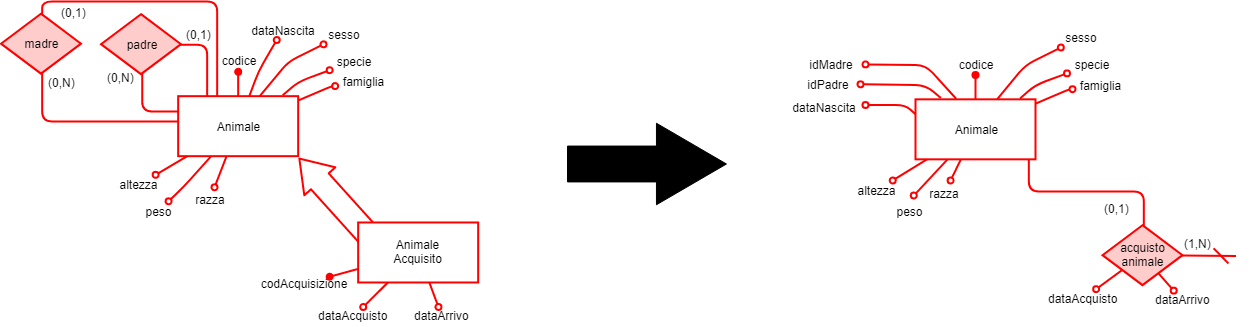
\includegraphics[scale=2, width=1.15\textwidth]{ridondanze/animale.png}
\caption{ge\-ne\-ra\-liz\-za\-zio\-ne dell'entità Animale Acquisito}
\end{figure}
La ge\-ne\-ra\-liz\-za\-zio\-ne dell'entità Animale Acquisito viene risolta sostituendo l'entità stessa con una relazione che mantiene gli stessi attributi ad eccezione del codice di acquisizione; essendo questa un' associazione con cardinalità (0,1)-(1,N), vengono utilizzati come chiave sia l'identificatore di animale che quello del fornitore. Ciò consente di eliminare i valori NULL per tutti i record di Animale relativi ad animali che non sono stati acquistati. Inoltre, vengono eliminate le relazioni ricorsive padre e madre tramite l'inserimento degli attributi \textit{idMadre} e \textit{idPadre} con vincoli di integrità referenziale.
\subsection{sensori}
\begin{figure}[H]
\centering
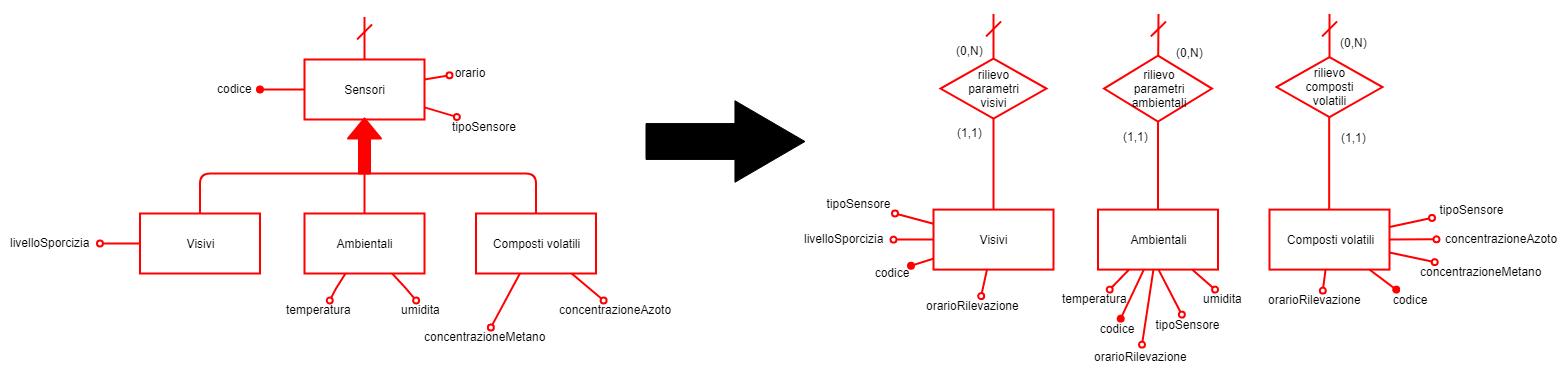
\includegraphics[scale=2, width=1.15\textwidth]{ridondanze/sensori.png}
\caption{ge\-ne\-ra\-liz\-za\-zio\-ne dell'entità Sensori}
\end{figure}
Si è preferito eliminare la ge\-ne\-ra\-liz\-za\-zio\-ne di Sensori dividendo l'entità in tre nuove entità indipendenti, in quanto ogni sensore raccoglie informazioni di tipo diverso, e ciò riempirebbe alternativamente la tabella di valori NULL. Con questa soluzione, ogni tipologia di sensore compila record completi e contenenti solamente i dati raccolti.
\subsection{acqua}
\begin{figure}[H]
\centering
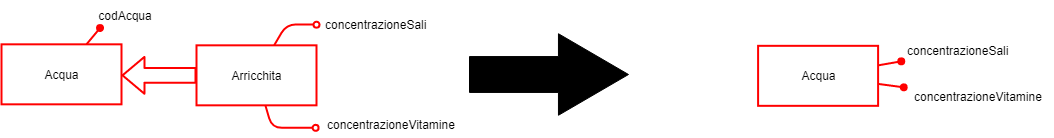
\includegraphics[scale=2, width=1.15\textwidth]{ridondanze/acqua.png}
\caption{ge\-ne\-ra\-liz\-za\-zio\-ne dell'entità Acqua Arricchita}
\end{figure}
La ge\-ne\-ra\-liz\-za\-zio\-ne parziale di Acqua Arricchita è stata eliminata considerando il fatto che trasformandola in una relazione si ottiene una tabella che contiene un solo attributo come chiave primaria. Questo non consente di avere informazioni dettagliate sull'acqua da fornire agli animali. Il problema si risolve utilizzando un'unica tabella che ha come identificatore primario le concentrazioni di vitamine e sali, considerando l'acqua non arricchita come avente concentrazioni pari a zero su entrambi gli attributi. Ciò consente di evitare valori NULL sulla chiave primaria.
\subsection{riproduzione}
\begin{figure}[H]
\centering
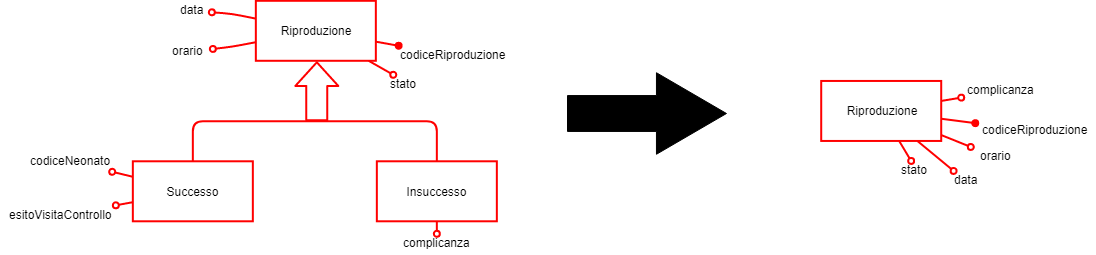
\includegraphics[scale=2, width=1.15\textwidth]{ridondanze/riproduzione.png}
\caption{ge\-ne\-ra\-liz\-za\-zio\-ne dell'entità Riproduzione}
\end{figure}
La ge\-ne\-ra\-liz\-za\-zio\-ne sulla tabella Riproduzione è stata ristrutturata considerando che entrambi gli attributi \textit{codiceNeonato} e \textit{esitoVisitaControllo} sono ridondanti e ricavabili tramite vincolo di integrità. Inoltre si è scelto di accorpare il campo delle complicanze a Riproduzione in quanto statisticamente i casi di insuccesso sono molto minori di quelli con successo, questo giustifica la presenza di alcuni valori NULL nella tabella Riproduzione, e consente di non creare due ulteriori entità nel database.
\subsection{allestimento}
\begin{figure}[H]
\centering
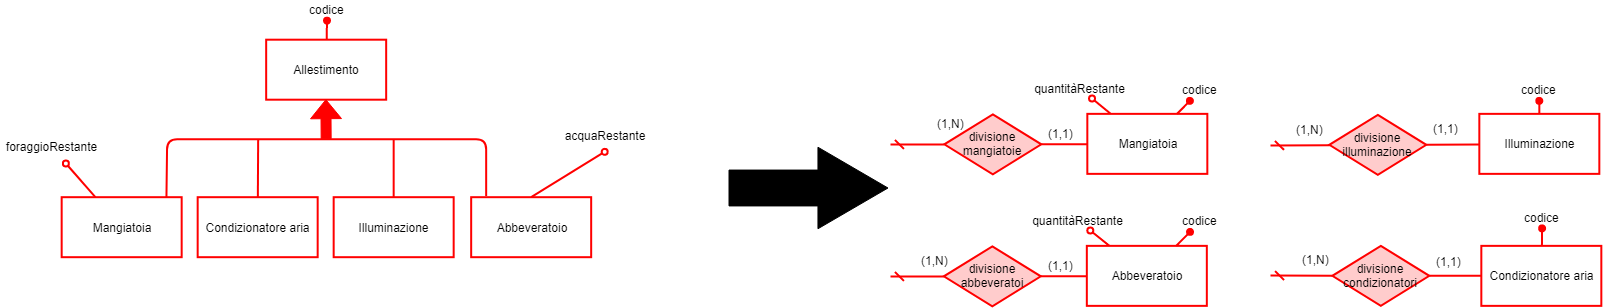
\includegraphics[scale=2, width=1.15\textwidth]{ridondanze/allestimento.png}
\caption{ge\-ne\-ra\-liz\-za\-zio\-ne dell'entità Allestimento}
\end{figure}
La ge\-ne\-ra\-liz\-za\-zio\-ne dell'entità Allestimento è stata risolta separando le varie entità figlie. Facendo ciò si eliminano i valori NULL sull'attributo \textit{quantitàRestante} per gli impianti di illuminazione e di condizionamento, inoltre si evita di controllare che i pasti vengano assegnati ad allestimenti non consoni (condizionamento e illuminazione).
\subsection{cliente}
\begin{figure}[H]
\centering
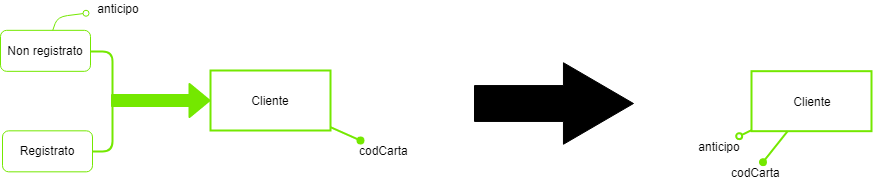
\includegraphics[scale=2, width=1.15\textwidth]{ridondanze/cliente.png}
\caption{ge\-ne\-ra\-liz\-za\-zio\-ne dell'entità Cliente Registrato}
\end{figure}
La ge\-ne\-ra\-liz\-za\-zio\-ne sulla registrazione dell'entità Cliente è stata risolta considerando solo l'entità stessa a cui è stato aggiunto l'attributo \textit{anticipo} derivato dall'entità figlia Non Registrato. Questo consente di ridurre il numero di tabelle nel database e di mantenere l'informazione inerente la registrazione del cliente azzerando il valore di \textit{anticipo} per tutti i clienti registrati.
\subsection{formaggio}
\begin{figure}[H]
\centering
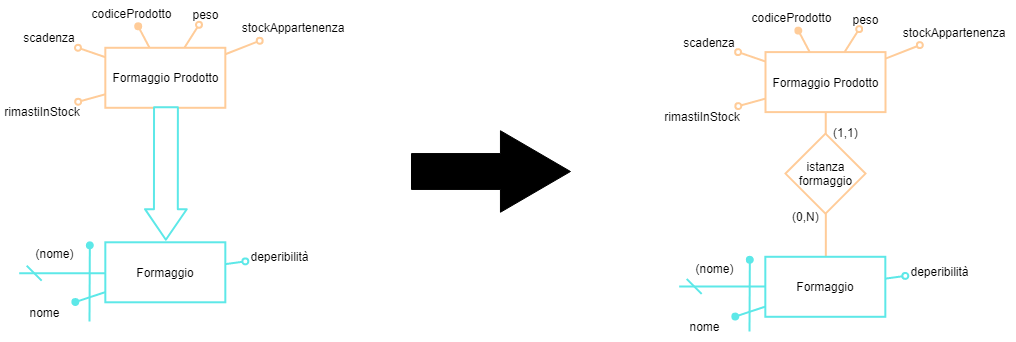
\includegraphics[scale=2, width=1.15\textwidth]{ridondanze/formaggio.png}
\caption{ge\-ne\-ra\-liz\-za\-zio\-ne dell'entità Formaggio Prodotto}
\end{figure}
Si è scelto di mantenere distinte le tabelle nella ge\-ne\-ra\-liz\-za\-zio\-ne di Formaggio, in quanto risulta importante la distinzione tra l'ipotetico prodotto di un singolo agriturismo e il formaggio effettivo (Formaggio Prodotto), che gode così di uno specifico lotto di appartenenza e una data di scadenza. Il prodotto potrà così essere fisicamente ordinato e recensito dai clienti.
\subsection{scheda medica}
\begin{figure}[H]
\centering
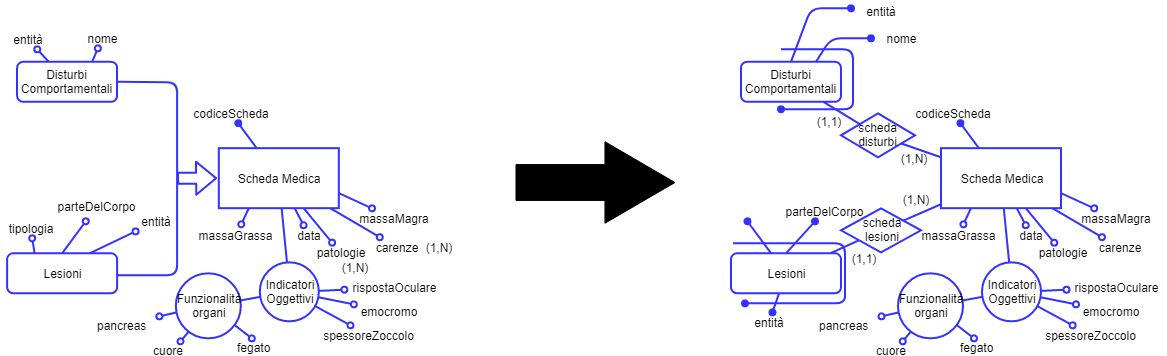
\includegraphics[scale=2, width=1.15\textwidth]{ridondanze/scheda_medica.png}
\caption{ge\-ne\-ra\-liz\-za\-zio\-ne dell'entità Scheda Medica}
\end{figure}
Si è scelto di mantenere distinte le entità figlie di Scheda Medica per mantenere le informazioni dei Disturbi Comportamentali e delle Lesioni separate. Così facendo si è evitata l'introduzione di molteplici valori NULL all'interno della tabella Scheda Medica.
\section{Individuazione delle Ridondanze}
\label{sec:ridondanze}
In questo capitolo vengono prese in esame tutte le informazioni ridondanti interne al database. Viene mostrato, inoltre, come è possibile eliminare le ridondanze superflue con la modifica o l'inserimento di nuovi attributi, oppure mantenere quelle utili per ricavare in modo semplice informazioni rilevanti e di frequente utilizzo, altrimenti difficilmente ricavabili.
\subsection{Ridondanze degli Attributi}
\label{subsec:ridondanze-attr}
\begin{itemize}

\item \`E stato tolto \textit{nome} da Fornitore in quanto ricavabile da \textit{ragione sociale}
\item \`E stato eliminato \textit{codice neonato} da Riproduzione in quanto ricavabile dal confronto tra \textit{id\_madre} e \textit{id\_padre} con \textit{codice madre} e \textit{codice padre} su coinvolge, tenendo conto della \textit{data} della specifica Riproduzione 
\item \`E stato eliminato \textit{stato} da Visita in quanto il valore di quest' attributo è ridondante rispetto alla presenza o no del valore NULL sull'attributo \textit{data effettiva}
\item \`E stato eliminato \textit{interventi di controllo programmati} da Scheda gestazione in quanto ricavabile verificando che la \textit{data programmata} di Visita sia successiva alla \textit{data} della Riproduzione, e che \textit{data effettiva} sia NULL
\item Si mantiene la ridondanza di \textit{capianza max} di Locale seppur possa essere ricavata dalla specie ospitata e dalle dimensioni dello stesso
\item Si mantiene le ridondanza delle \textit{kcal/kg} del Foraggio seppur possa essere ricavata dalle quantità di fibre, proteine e glucidi contenute
\item Si mantiene il \textit{nome} ed il \textit{cognome} dei Veterinari seppur possano essere ricavati dal \textit{codice fiscale}
\item Si mantiene il \textit{nome} ed il \textit{cognome} degli Account seppur possano essere ricavati dal \textit{codice fiscale}
\item Si mantiene la \textit{scadenza} del Formaggio Prodotto seppur possa essere ricavata dalla \textit{deperibilità} del Formaggio insieme alla \textit{data di produzione} del Lotto associato
\item Si mantiene il \textit{totale da pagare} nei Pagamenti seppur ricavabile come somma di tutti i costi delle camere, delle escursioni e dei servizi aggiuntivi: ciò permette di centralizzare l'informazione del pagamento totale in un unica tabella
\end{itemize}

\subsection{Ridondanze E-R}
\label{subsec:ridondanze-ent-rel}

\begin{enumerate}

\item \`E stata introdotta la ridondanza \textit{pasto per mangiatoia}
\item \`E stata introdotta la ridondanza \textit{pasto per abbeveratoio}
\item \`E stata introdotta la ridondanza \textit{qualità pasto}
\item \`E stata introdotta la ridondanza \textit{controllo qualità}
%\item è stata rimossa la relazione \textit{controlli effettuati} tra Riproduzione e Visita, in quanto si introduceva una ridondanza su una parte più ristretta dei record di Visita, in particolare si potevano ricavare solo le visite conseguenti una riproduzione.
%\item è stata introdotta la relazione \textit{appartenenza agriturismo} tra Zona pascolo e Agriturismo al fine di ricavare in che agriturismo si trova ogni animale che sta pascolando, sfruttando i dati del GPS, ed eventualmente riconoscere possibili animali "sperduti". Questo aumenta anche l'efficienza dell'operazione in quanto diminuisce il numero di accessi dovuti alle letture e scritture di tabelle intermedie (Locale, stalla, Attività pascolo, etc.) tra Agriturismo e Zona di Pascolo 

\end{enumerate}

\newpage
\section{Analisi delle Operazioni}
\label{sec:operazioni}
Sono qui illustrate le principali operazioni significative capaci di apportare un forte contributo al carico applicativo della base di dati.
Di ciascuna viene data una breve descrizione, assieme ad una stima della frequenza giornaliera con cui verranno svolte.
Questo permetterà, assieme ai volumi stimati per ogni entità e relazione nel sistema (riportati a partire da pag. \pageref{sec:volumi}), di derivare il carico effettivo che il database dovrà gestire in termini di operazioni elementari, quali scritture e letture.
\subsection{Operazioni}
\begin{enumerate}
\item \textbf{Aggiornamento riproduzione}
	\begin{itemize}
	\item \textit{Descrizione: }L'operazione produce due aggiornamenti, all'inserimento di una nuova riproduzione e al suo completamento. Il primo compila un nuovo record di Riproduzione assieme ai dati del veterinario supervisore. Il secondo aggiorna lo stato della riproduzione e compila una scheda di gestazione con le relative visite di controllo programmate. Infine, in caso di successo, vengono registrati i dati anagrafici del nuovo animale, il gps a cui è associato e le informazioni riguardanti il locale abitato.
	\item \textit{Frequenza: } 1 volta al giorno
	\end{itemize}
\item \textbf{Recupero delle visite di controllo programmate}
	\begin{itemize}
	\item \textit{Descrizione: }Permette di estrarre tutte le visite di controllo programmate per un determinato animale
	\item \textit{Frequenza: }55 volte al giorno (per controllare tutti gli animali della rete in un anno)
	\end{itemize}
\item \textbf{Gestione dei pagamenti}
	\begin{itemize}
	\item \textit{Descrizione: }Ogni giorno, ogni agriturismo gestisce i pagamenti di tre clienti che hanno usufruito delle escursioni o delle camere con servizi aggiuntivi disponibili.
	\item \textit{Frequenza: }60 volte al giorno
	\end{itemize}
\item \textbf{Inserimento e modifica degli account}
	\begin{itemize}
	\item \textit{Descrizione: }La rete gestisce mediamente l'inserimento o la modifica di venti account ogni giorno
	\item \textit{Frequenza: }20 volte al giorno
	\end{itemize}
\item \textbf{Stoccaggio del latte}
	\begin{itemize}
	\item \textit{Descrizione: }Ogni giorno, ogni agriturismo gestisce la mungitura e il corretto stoccaggio di circa dieci tipologie diverse di latte
	\item \textit{Frequenza: }200 volte al giorno
	\end{itemize}
\item \textbf{Controlli dell'igiene dei locali}
	\begin{itemize}
	\item \textit{Descrizione: }Ogni giorno vengono controllati tutti i parametri di due locali di ogni agriturismo affinché rientrino nelle soglie di tollerabilità; in caso contrario viene effettuata una richiesta d'intervento di pulizia
	\item \textit{Frequenza: }40 volte al giorno
	\end{itemize}
\item \textbf{Calcolo apporto calorico dei pasti}
	\begin{itemize}
	\item \textit{Descrizione: }Ogni giorno vengono controllati tutti e tre i pasti di ogni locale di ogni agriturismo affinché si conoscano i corretti valori di apporto calorico somministrati agli animali
	\item \textit{Frequenza: }1500 volte al giorno
	\end{itemize}
\item \textbf{Processamento degli ordini}
	\begin{itemize}
	\item \textit{Descrizione: }Ogni giorno ogni agriturismo gestisce mediamente cento ordini effettuati dai clienti registrati nello store online
	\item \textit{Frequenza: }2000 volte al giorno
	\end{itemize}
\item \textbf{Prescrizione delle terapie}
	\begin{itemize}
	\item \textit{Descrizione: }Ogni giorno, ogni agriturismo riceve mediamente tre nuove terapie per i propri animali da parte dei veterinari addetti
	\item \textit{Frequenza: }60 volte al giorno
	\end{itemize}
\item \textbf{Controllo animali dispersi}
	\begin{itemize}
	\item \textit{Descrizione: }Durante le otto ore disponibili per il pascolo, ogni animale viene controllato ogni venti minuti affinché la sua posizione non sconfini in una zona di pascolo di un altro agriturismo.
	\item \textit{Frequenza: }24 volte al giorno
	\end{itemize}

\end{enumerate}

\subsection{Tavole dei Volumi}
\label{sec:volumi}


\subsubsection{Area Allevamento}
\begin{center}
\setlength{\extrarowheight}{1.5pt}
\begin{longtable}{|p{0.23\linewidth}|p{0.1\linewidth}|p{0.11\linewidth}|p{0.45\linewidth}|}
\hline \textbf{Nome} 	& \begin{center}\vspace{-15pt}\textbf{E/R}\end{center} & \textbf{Numero Istanze} & \textbf{Motivazione}\\ 

    
\hline
Acqua 				& \begin{center}
\vspace{-25pt}E
\end{center}
					& \begin{center}
					\vspace{-25pt}20\end{center}
					& \begin{flushleft}\vspace{-25pt} Si considerano circa 20 tipologie uniche di acqua \end{flushleft}\\ 

\hline
Agriturismo 				& \begin{center}
\vspace{-25pt}E
\end{center}
					& \begin{center}
					\vspace{-25pt}20
					\end{center}
					& \begin{flushleft}\vspace{-25pt} Ipotesi iniziale \end{flushleft}\\ 

\hline
Allestimento 				& \begin{center}
\vspace{-25pt}E
\end{center}
					& \begin{center}
					\vspace{-25pt}4000\end{center}
					& \begin{flushleft}\vspace{-25pt} Ogni locale è provvisto mediamente di otto allestimenti: due mangiatoie, due abbeveratoi, due dispositivi per il condizionamento dell'aria e due sistemi di illuminazione $8\times 500 = 4000$\end{flushleft}\\ 

\hline
Ambientali 				& \begin{center}
\vspace{-25pt}E
\end{center}
					& \begin{center}
					\vspace{-25pt}500\end{center}
					& \begin{flushleft}\vspace{-25pt} Ogni locale è dotato di un sensore per i parametri ambientali \end{flushleft}\\ 

\hline
Animale 				& \begin{center}
\vspace{-25pt}E
\end{center}
					& \begin{center}
					\vspace{-25pt}20000\end{center}
					& \begin{flushleft}\vspace{-25pt} Ogni agriturismo ospita 1000 animali $20\times 1000=20000$ \end{flushleft}\\ 

\hline
Area pascolo 				& \begin{center}
\vspace{-25pt}E
\end{center}
					& \begin{center}
					\vspace{-25pt}60\end{center}
					& \begin{flushleft}\vspace{-25pt} Ogni agriturismo dispone di 3 aree di pascolo $3\times 20= 60$\end{flushleft}\\ 

\hline
Attività pascolo 				& \begin{center}
\vspace{-25pt}E
\end{center}
					& \begin{center}
					\vspace{-25pt}4500\end{center}
					& \begin{flushleft}\vspace{-25pt} Mediamente, ogni agriturismo dispone delle proprie 3 aree di pascolo e altre 6 degli agriturismi limitrofi $500\times 9 = 4500$\end{flushleft}\\ 

\hline
Composti volatili 				& \begin{center}
\vspace{-25pt}E
\end{center}
					& \begin{center}
					\vspace{-25pt}500\end{center}
					& \begin{flushleft}\vspace{-25pt} Ogni locale è dotato di un sensore per i composti volatili \end{flushleft}\\ 

\hline
Foraggio 				& \begin{center}
\vspace{-25pt}E
\end{center}
					& \begin{center}
					\vspace{-25pt}50\end{center}
					& \begin{flushleft}\vspace{-25pt} Si considerano circa 50 tipologie uniche di foraggio \end{flushleft}\\ 

\hline
Fornitore 				& \begin{center}
\vspace{-25pt}E
\end{center}
					& \begin{center}
					\vspace{-25pt}20\end{center}
					& \begin{flushleft}\vspace{-25pt} Si assume una media di un fornitore per agriturismo \end{flushleft}\\ 

\hline
GPS 				& \begin{center}
\vspace{-25pt}E
\end{center}
					& \begin{center}
					\vspace{-25pt}20000\end{center}
					& \begin{flushleft}\vspace{-25pt} Ogni animale è dotato di un dispositivo GPS \end{flushleft}\\ 

\hline
Locale 				& \begin{center}
\vspace{-25pt}E
\end{center}
					& \begin{center}
					\vspace{-25pt}500\end{center}
					& \begin{flushleft}\vspace{-25pt} Ogni stalla ha in media 5 locali \end{flushleft}\\ 

\hline
Pasto 				& \begin{center}
\vspace{-25pt}E
\end{center}
					& \begin{center}
					\vspace{-25pt}1000\end{center}
					& \begin{flushleft}\vspace{-25pt} Combinazione tra tutti i tipi di acqua e di foraggio $20\times 50= 1000$ \end{flushleft}\\ 

\hline
Pasto per Locale 				& \begin{center}
\vspace{-25pt}R
\end{center}
					& \begin{center}
					\vspace{-25pt}547500\end{center}
					& \begin{flushleft}\vspace{-25pt} Tre pasti al giorno per un anno per ogni locale $3\times365\times500=547500$ \end{flushleft}\\ 

\hline
Pulizia locale 				& \begin{center}
\vspace{-25pt}E
\end{center}
					& \begin{center}
					\vspace{-25pt}580\end{center}
					& \begin{flushleft}\vspace{-25pt} Ogni agriturismo effettua due richieste al giorno, per un totale di $2\times 365=730$ richieste annue. In questo modo, ognuno dei 25 locali viene pulito ${730\over 25}=29$ volte l'anno. Quindi i 20 agriturismi compilano $29\times 20=580$ record all'anno. \end{flushleft}\\ 

\hline
Recinzione divisoria e zona di pascolo 				& \begin{center}
\vspace{-25pt}E
\end{center}
					& \begin{center}
					\vspace{-25pt}180\end{center}
					& \begin{flushleft}\vspace{-25pt} Ogni area di pascolo è divisa in 3 recinsioni $60\times 3= 180$\end{flushleft}\\ 

\hline
Riproduzione 				& \begin{center}
\vspace{-25pt}E
\end{center}
					& \begin{center}
					\vspace{-25pt}12900\end{center}
					& \begin{flushleft}\vspace{-25pt} Secondo l'Istat circa il $75\%$ degli animali è femmina, nel nostro caso $20000\times0.75=15000$. Di queste, il $14\%$ non è destinato all'allevamento, quindi in un anno il restante $86\%$ si riproduce $15000\times 0.86=12900$ \end{flushleft}\\ 

\hline
Scheda gestazione 				& \begin{center}
\vspace{-25pt}E
\end{center}
					& \begin{center}
					\vspace{-25pt}11610\end{center}
					& \begin{flushleft}\vspace{-25pt} Viene generata una nuova scheda di gestazione per ogni riproduzione andata a buon fine, ossia il $90\%$ delle riproduzioni $12900\times 0.9= 11610$\end{flushleft}\\ 

\hline
Stalla 				& \begin{center}
\vspace{-25pt}E
\end{center}
					& \begin{center}
					\vspace{-25pt}100\end{center}
					& \begin{flushleft}\vspace{-25pt} Ogni agriturismo possiede in media 5 stalle \end{flushleft}\\ 

\hline
Visivi 				& \begin{center}
\vspace{-25pt}E
\end{center}
					& \begin{center}
					\vspace{-25pt}500\end{center}
					& \begin{flushleft}\vspace{-25pt} Ogni locale è dotato di un sensore per i parametri visivi \end{flushleft}\\ 

\hline
abita 				& \begin{center}
\vspace{-25pt}R
\end{center}
					& \begin{center}
					\vspace{-25pt}20000\end{center}
					& \begin{flushleft}\vspace{-25pt} Cardinalità (1,1) con Animale \end{flushleft}\\ 

\hline
acquisto animale 				& \begin{center}
\vspace{-25pt}R
\end{center}
					& \begin{center}
					\vspace{-25pt}10000\end{center}
					& \begin{flushleft}\vspace{-25pt} Cardinalità (1,1) con ogni animale acquisito, ossia con il $50\%$ del voume di Animali \end{flushleft}\\ 

\hline
%appartenenza agriturismo 				& \begin{center}
%\vspace{-25pt}R
%\end{center}
%					& \begin{center}
%					\vspace{-25pt}180\end{center}
%					& \begin{flushleft}\vspace{-25pt} Cardinalità (1,1) con Recinzione divisoria e zona di pascolo \end{flushleft}\\ 
%
%\hline
attività locale 				& \begin{center}
\vspace{-25pt}R
\end{center}
					& \begin{center}
					\vspace{-25pt}30000\end{center}
					& \begin{flushleft}\vspace{-25pt} Cardinalità (1,1) con Attività pascolo \end{flushleft}\\ 

\hline
coinvolge 				& \begin{center}
\vspace{-25pt}R
\end{center}
					& \begin{center}
					\vspace{-25pt}12900\end{center}
					& \begin{flushleft}\vspace{-25pt} Cardinalità (1,1) con Riproduzione \end{flushleft}\\ 

\hline
collocazione attività 				& \begin{center}
\vspace{-25pt}R
\end{center}
					& \begin{center}
					\vspace{-25pt}4500\end{center}
					& \begin{flushleft}\vspace{-25pt} Cardinalità (1,1) con Attività pascolo \end{flushleft}\\ 

\hline
composizione acqua 				& \begin{center}
\vspace{-25pt}R
\end{center}
					& \begin{center}
					\vspace{-25pt}1000\end{center}
					& \begin{flushleft}\vspace{-25pt} Cardinalità (1,1) con Pasto \end{flushleft}\\ 

\hline
composizione foraggio 				& \begin{center}
\vspace{-25pt}R
\end{center}
					& \begin{center}
					\vspace{-25pt}1000\end{center}
					& \begin{flushleft}\vspace{-25pt} Cardinalità (1,1) con Pasto \end{flushleft}\\ 

\hline
composizione pasto 				& \begin{center}
\vspace{-25pt}R
\end{center}
					& \begin{center}
					\vspace{-25pt}12000\end{center}
					& \begin{flushleft}\vspace{-25pt} Ogni locale cambia pasto circa 24 volte l'anno $500\times 24= 12000$ \end{flushleft}\\ 

\hline
determina 				& \begin{center}
\vspace{-25pt}R
\end{center}
					& \begin{center}
					\vspace{-25pt}11610\end{center}
					& \begin{flushleft}\vspace{-25pt} Cardinalità (1,1) con Scheda gestazione \end{flushleft}\\ 

\hline
divisione allestimento 				& \begin{center}
\vspace{-25pt}R
\end{center}
					& \begin{center}
					\vspace{-25pt}4000\end{center}
					& \begin{flushleft}\vspace{-25pt} Cardinalità (1,1) con Allestimento \end{flushleft}\\ 

\hline
divisione locale 				& \begin{center}
\vspace{-25pt}R
\end{center}
					& \begin{center}
					\vspace{-25pt}500\end{center}
					& \begin{flushleft}\vspace{-25pt} Cardinalità (1,1) con Locale \end{flushleft}\\ 

\hline
divisione pascolo 				& \begin{center}
\vspace{-25pt}R
\end{center}
					& \begin{center}
					\vspace{-25pt}180\end{center}
					& \begin{flushleft}\vspace{-25pt} Cardinalità (1,1) con Recinzione divisoria e zona di pascolo \end{flushleft}\\ 

\hline
divisione stalle 				& \begin{center}
\vspace{-25pt}R
\end{center}
					& \begin{center}
					\vspace{-25pt}100\end{center}
					& \begin{flushleft}\vspace{-25pt} Cardinalità (1,1) con Stalla \end{flushleft}\\ 

\hline
locale assegnato 				& \begin{center}
\vspace{-25pt}R
\end{center}
					& \begin{center}
					\vspace{-25pt}547500\end{center}
					& \begin{flushleft}\vspace{-25pt} Cardinalità (1,1) con Pasto per Locale \end{flushleft}\\ 

\hline
localizzato 				& \begin{center}
\vspace{-25pt}R
\end{center}
					& \begin{center}
					\vspace{-25pt}20000\end{center}
					& \begin{flushleft}\vspace{-25pt} Cardinalità (1,1) con Animale e con GPS \end{flushleft}\\ 

\hline
pasto assegnato 				& \begin{center}
\vspace{-25pt}R
\end{center}
					& \begin{center}
					\vspace{-25pt}547500\end{center}
					& \begin{flushleft}\vspace{-25pt} Cardinalità (1,1) con Pasto per Locale \end{flushleft}\\ 

\hline
richiesta intervento 				& \begin{center}
\vspace{-25pt}R
\end{center}
					& \begin{center}
					\vspace{-25pt}580\end{center}
					& \begin{flushleft}\vspace{-25pt} Cardinalità (1,1) con Pulizia locale \end{flushleft}\\ 

\hline
rilievo composti volatili 				& \begin{center}
\vspace{-25pt}R
\end{center}
					& \begin{center}
					\vspace{-25pt}500\end{center}
					& \begin{flushleft}\vspace{-25pt} Cardinalità (1,1) con Composti volatili \end{flushleft}\\ 

\hline
rilievo parametri ambientali 				& \begin{center}
\vspace{-25pt}R
\end{center}
					& \begin{center}
					\vspace{-25pt}500\end{center}
					& \begin{flushleft}\vspace{-25pt} Cardinalità (1,1) con rilievo parametri ambientali \end{flushleft}\\ 

\hline
rilievo parametri visivi 				& \begin{center}
\vspace{-25pt}R
\end{center}
					& \begin{center}
					\vspace{-25pt}500\end{center}
					& \begin{flushleft}\vspace{-25pt} Cardinalità (1,1) con Visivi \end{flushleft}\\ 

\hline
scrive 				& \begin{center}
\vspace{-25pt}R
\end{center}
					& \begin{center}
					\vspace{-25pt}11610\end{center}
					& \begin{flushleft}\vspace{-25pt} Cardinalità (1,1) con Scheda gestazione \end{flushleft}\\ 

\hline
supervisiona 				& \begin{center}
\vspace{-25pt}R
\end{center}
					& \begin{center}
					\vspace{-25pt}12900\end{center}
					& \begin{flushleft}\vspace{-25pt} Cardinalità (1,1) con Riproduzione \end{flushleft}\\ 

\hline

\end{longtable}\end{center}


\subsubsection{Area Healthcare}
\begin{center}\setlength{\extrarowheight}{1.5pt}\begin{longtable}{|p{0.23\linewidth}|p{0.1\linewidth}|p{0.11\linewidth}|p{0.45\linewidth}|}
\hline \textbf{Nome}   & \begin{center}\vspace{-15pt}\textbf{E/R}\end{center} & \textbf{Numero Istanze} & \textbf{Motivazione}\\ 

    
\hline
Esame
 & 
\begin{center}\vspace{-25pt}E\end{center}
 & 
\begin{center}\vspace{-25pt}8000\end{center}
 & 
\begin{flushleft}\vspace{-25pt}Per ogni agriturismo vengono prescritti una media di 400 esami l'anno per un totale di 8000 esami\end{flushleft}
\\

\hline
Farmaco
 & 
\begin{center}\vspace{-25pt}E\end{center}
 & 
\begin{center}\vspace{-25pt}100\end{center}
 & 
\begin{flushleft}\vspace{-25pt}Si suppone che le malattie vengano curate con l'utilizzo di 100 farmaci diversi utilizzati in tutta la rete di \textit{Farmhouse 4.0}\end{flushleft}
\\

\hline
Indici Salute
 & 
\begin{center}\vspace{-25pt}E\end{center}
 & 
\begin{center}\vspace{-25pt}22000\end{center}
 & 
\begin{flushleft}\vspace{-25pt}Per ogni visita vengono rilevati nuovamente gli indici di salute\end{flushleft}
\\

\hline
Scheda Medica
 & 
\begin{center}\vspace{-25pt}E\end{center}
 & 
\begin{center}\vspace{-25pt}40000\end{center}
 & 
\begin{flushleft}\vspace{-25pt}Si suppone che in un anno siano registrate 40000 schede\end{flushleft}
\\

\hline
Terapia
 & 
\begin{center}\vspace{-25pt}E\end{center}
 & 
\begin{center}\vspace{-25pt}2000\end{center}
 & 
\begin{flushleft}\vspace{-25pt}Si suppone che ogni anno vengano prescritte 100 terapie per ogni agriturismo $100\times 20= 2000$\end{flushleft}
\\

\hline
Veterinario
 & 
\begin{center}\vspace{-25pt}E\end{center}
 & 
\begin{center}\vspace{-25pt}100\end{center}
 & 
\begin{flushleft}\vspace{-25pt}Si suppone che ogni agriturismo sia controllato da cinque veterinari $20\times 5= 100$\end{flushleft}
\\

\hline
Visita
 & 
\begin{center}\vspace{-25pt}E\end{center}
 & 
\begin{center}\vspace{-25pt}22000\end{center}
 & 
\begin{flushleft}\vspace{-25pt}Si suppone che per ogni agriturismo vengano eseguite 1100 visite all'anno per poter controllare almeno una volta tutti gli animali $1100\times 20= 22000$\end{flushleft}
\\

\hline
compila
 & 
\begin{center}\vspace{-25pt}R\end{center}
 & 
\begin{center}\vspace{-25pt}40000\end{center}
 & 
\begin{flushleft}\vspace{-25pt}Cardinalità (1,1) con Scheda Medica\end{flushleft}
\\

\hline
composta da
 & 
\begin{center}\vspace{-25pt}R\end{center}
 & 
\begin{center}\vspace{-25pt}6000\end{center}
 & 
\begin{flushleft}\vspace{-25pt}Ogni terapia impiega circa 3 farmaci diversi $2000\times 3 = 6000$\end{flushleft}
\\

\hline
controlli effettuati
 & 
\begin{center}\vspace{-25pt}R\end{center}
 & 
\begin{center}\vspace{-25pt}12900\end{center}
 & 
\begin{flushleft}\vspace{-25pt}Viene effettuata una visita di controllo per ogni riproduzione con successo o insuccesso  \end{flushleft}
\\

\hline
esegue
 & 
\begin{center}\vspace{-25pt}R\end{center}
 & 
\begin{center}\vspace{-25pt}22000\end{center}
 & 
\begin{flushleft}\vspace{-25pt}Cardinalità (1,1) con Visita\end{flushleft}
\\

\hline
possiede
 & 
\begin{center}\vspace{-25pt}R\end{center}
 & 
\begin{center}\vspace{-25pt}40000\end{center}
 & 
\begin{flushleft}\vspace{-25pt}Cardinalità (1,1) con Scheda Medica\end{flushleft}
\\

\hline
possiede esame
 & 
\begin{center}\vspace{-25pt}R\end{center}
 & 
\begin{center}\vspace{-25pt}8000\end{center}
 & 
\begin{flushleft}\vspace{-25pt}Cardinalità (1,1) con Esame\end{flushleft}
\\

\hline
possiede terapia
 & 
\begin{center}\vspace{-25pt}R\end{center}
 & 
\begin{center}\vspace{-25pt}2000\end{center}
 & 
\begin{flushleft}\vspace{-25pt}Cardinalità (1,1) con Terapia\end{flushleft}
\\

\hline
prescrive
 & 
\begin{center}\vspace{-25pt}R\end{center}
 & 
\begin{center}\vspace{-25pt}2000\end{center}
 & 
\begin{flushleft}\vspace{-25pt}Cardinalità (1,1) con Terapia\end{flushleft}
\\

\hline
prescrive esame
 & 
\begin{center}\vspace{-25pt}R\end{center}
 & 
\begin{center}\vspace{-25pt}8000\end{center}
 & 
\begin{flushleft}\vspace{-25pt}Cardinalità (1,1) con Esame\end{flushleft}
\\

\hline
stato salute
 & 
\begin{center}\vspace{-25pt}R\end{center}
 & 
\begin{center}\vspace{-25pt}22000\end{center}
 & 
\begin{flushleft}\vspace{-25pt}Cardinalità (1,1) con Indici Salute\end{flushleft}
\\

\hline

\end{longtable}\end{center}


\subsubsection{Area Produzione}
\begin{center}
\setlength{\extrarowheight}{1.5pt}
\begin{longtable}{|p{0.23\linewidth}|p{0.1\linewidth}|p{0.11\linewidth}|p{0.45\linewidth}|}
\hline \textbf{Nome} 	& \begin{center}\vspace{-15pt}\textbf{E/R}\end{center} & \textbf{Numero Istanze} & \textbf{Motivazione}\\ 

    
\hline
Cantine 				& \begin{center}
\vspace{-25pt}E
\end{center}
					& \begin{center}
					\vspace{-25pt}100\end{center}
					& \begin{flushleft}\vspace{-25pt} Mediamente sono disponibili 5 cantine per ogni agriturismo $20\times 5=100$ \end{flushleft}\\ 

\hline
Fasi 				& \begin{center}
\vspace{-25pt}E
\end{center}
					& \begin{center}
					\vspace{-25pt}4000\end{center}
					& \begin{flushleft}\vspace{-25pt} Ogni ricetta è divisa mediamente in 10 fasi $400\times 10 = 4000$\end{flushleft}\\ 

\hline
Formaggio 				& \begin{center}
\vspace{-25pt}E
\end{center}
					& \begin{center}
					\vspace{-25pt}400\end{center}
					& \begin{flushleft}\vspace{-25pt} Ogni agriturismo produce circa 20 formaggi differenti \end{flushleft}\\ 

\hline
Latte 				& \begin{center}
\vspace{-25pt}E
\end{center}
					& \begin{center}
					\vspace{-25pt}400\end{center}
					& \begin{flushleft}\vspace{-25pt} Ogni agriturismo produce 20 tipologie di latte differente $20\times 20 = 400$\end{flushleft}\\ 

\hline
Lotto 				& \begin{center}
\vspace{-25pt}E
\end{center}
					& \begin{center}
					\vspace{-25pt}400\end{center}
					& \begin{flushleft}\vspace{-25pt} Ogni agriturismo produce 20 lotti di formaggio all'anno \end{flushleft}\\ 

\hline
Magazzini 				& \begin{center}
\vspace{-25pt}E
\end{center}
					& \begin{center}
					\vspace{-25pt}100\end{center}
					& \begin{flushleft}\vspace{-25pt} Mediamente sono disponibili 5 magazzini per ogni agriturismo $20\times 5 = 100$ \end{flushleft}\\ 

\hline
Mungitrice 				& \begin{center}
\vspace{-25pt}E
\end{center}
					& \begin{center}
					\vspace{-25pt}2000\end{center}
					& \begin{flushleft}\vspace{-25pt} Ogni agriturismo dispone di circa 100 mungitrici $20\times 100= 2000$ \end{flushleft}\\ 

\hline
Mungitura 				& \begin{center}
\vspace{-25pt}E
\end{center}
					& \begin{center}
					\vspace{-25pt}7300000\end{center}
					& \begin{flushleft}\vspace{-25pt} Si suppone che ogni giorno dell'anno ogni animale di un agriturismo venga munto una volta $20000\times 365 = 7300000$ \end{flushleft}\\ 

\hline
Parametri 				& \begin{center}
\vspace{-25pt}E
\end{center}
					& \begin{center}
					\vspace{-25pt}36500\end{center}
					& \begin{flushleft}\vspace{-25pt} Ogni giorno dell'anno vengono prelevati i parametri di tutte le cantine $365\times 100= 36500$ \end{flushleft}\\ 

\hline
Ricetta 				& \begin{center}
\vspace{-25pt}E
\end{center}
					& \begin{center}
					\vspace{-25pt}400\end{center}
					& \begin{flushleft}\vspace{-25pt} Si considerano circa 400 ricette differenti \end{flushleft}\\ 

\hline
Scaffalature 				& \begin{center}
\vspace{-25pt}E
\end{center}
					& \begin{center}
					\vspace{-25pt}1000\end{center}
					& \begin{flushleft}\vspace{-25pt} Ogni cantina è suddivisa in 10 scaffalature \end{flushleft}\\ 

\hline
Scaffali 				& \begin{center}
\vspace{-25pt}E
\end{center}
					& \begin{center}
					\vspace{-25pt}1000\end{center}
					& \begin{flushleft}\vspace{-25pt} Ogni magazzino è suddiviso in 10 scaffali $100\times 10=1000$\end{flushleft}\\ 

\hline
Silos 				& \begin{center}
\vspace{-25pt}E
\end{center}
					& \begin{center}
					\vspace{-25pt}200\end{center}
					& \begin{flushleft}\vspace{-25pt} Sono disponibili circa 10 silos per ogni agriturismo $10\times 20=200$ \end{flushleft}\\ 

\hline
appartenente a 				& \begin{center}
\vspace{-25pt}R
\end{center}
					& \begin{center}
					\vspace{-25pt}3000000\end{center}
					& \begin{flushleft}\vspace{-25pt} Cardinalità (1,1) con Formaggio Prodotto \end{flushleft}\\ 

\hline
che munge 				& \begin{center}
\vspace{-25pt}R
\end{center}
					& \begin{center}
					\vspace{-25pt}800000\end{center}
					& \begin{flushleft}\vspace{-25pt} Combinazione tra tutte le mungitrici e tutti i tipi di latte $2000\times 400= 800000$ \end{flushleft}\\ 

\hline
composizione formaggio 				& \begin{center}
\vspace{-25pt}R
\end{center}
					& \begin{center}
					\vspace{-25pt}400\end{center}
					& \begin{flushleft}\vspace{-25pt} Cardinalità (1,1) con Formaggio \end{flushleft}\\ 

\hline
con 				& \begin{center}
\vspace{-25pt}R
\end{center}
					& \begin{center}
					\vspace{-25pt}7300000\end{center}
					& \begin{flushleft}\vspace{-25pt} Cardinalità (1,1) con Mungitura \end{flushleft}\\ 

\hline
contengono scaffalature 				& \begin{center}
\vspace{-25pt}R
\end{center}
					& \begin{center}
					\vspace{-25pt}1000\end{center}
					& \begin{flushleft}\vspace{-25pt} Cardinalità (1,1) con Scaffalature \end{flushleft}\\ 

\hline
contengono scaffali 				& \begin{center}
\vspace{-25pt}R
\end{center}
					& \begin{center}
					\vspace{-25pt}1000\end{center}
					& \begin{flushleft}\vspace{-25pt} Cardinalità (1,1) con Scaffali \end{flushleft}\\ 

\hline
controllo fasi 				& \begin{center}
\vspace{-25pt}R
\end{center}
					& \begin{center}
					\vspace{-25pt}4000\end{center}
					& \begin{flushleft}\vspace{-25pt} Combinazione tra tutti i lotti e le proprie 10 fasi di produzione $400\times 10=4000$ \end{flushleft}\\ 

\hline
divisa in 				& \begin{center}
\vspace{-25pt}R
\end{center}
					& \begin{center}
					\vspace{-25pt}4000\end{center}
					& \begin{flushleft}\vspace{-25pt} Ogni ricetta è divisa in 10 fasi $400\times 10= 4000$\end{flushleft}\\ 

\hline
prodotto con 				& \begin{center}
\vspace{-25pt}R
\end{center}
					& \begin{center}
					\vspace{-25pt}160000\end{center}
					& \begin{flushleft}\vspace{-25pt} Combinazione tra tutti i tipi di latte e tutti i lotti $400\times 400 = 160000$\end{flushleft}\\ 

\hline
produce 				& \begin{center}
\vspace{-25pt}R
\end{center}
					& \begin{center}
					\vspace{-25pt}400\end{center}
					& \begin{flushleft}\vspace{-25pt} Cardinalità (1,1) con Formaggio \end{flushleft}\\ 

\hline
produce 				& \begin{center}
\vspace{-25pt}R
\end{center}
					& \begin{center}
					\vspace{-25pt}400\end{center}
					& \begin{flushleft}\vspace{-25pt} Cardinalità (1,1) con Latte \end{flushleft}\\ 

\hline
rilievo parametri 				& \begin{center}
\vspace{-25pt}R
\end{center}
					& \begin{center}
					\vspace{-25pt}36500\end{center}
					& \begin{flushleft}\vspace{-25pt} Cardinalità (1,1) con Parametri \end{flushleft}\\ 

\hline
stoccaggio cantine 				& \begin{center}
\vspace{-25pt}R
\end{center}
					& \begin{center}
					\vspace{-25pt}2000\end{center}
					& \begin{flushleft}\vspace{-25pt} Ogni agriturismo stocca 20 lotti nelle proprie 5 cantine $20\times 20 \times 5 = 2000$ \end{flushleft}\\ 

\hline
stoccaggio magazzini 				& \begin{center}
\vspace{-25pt}R
\end{center}
					& \begin{center}
					\vspace{-25pt}2000\end{center}
					& \begin{flushleft}\vspace{-25pt} Ogni agriturismo stocca 20 lotti nei propri 5 magazzini $20\times 20 \times 5 = 2000$ \end{flushleft}\\ 

\hline
stoccato in 				& \begin{center}
\vspace{-25pt}R
\end{center}
					& \begin{center}
					\vspace{-25pt}400\end{center}
					& \begin{flushleft}\vspace{-25pt} Cardinalità (1,1) con Latte \end{flushleft}\\ 

\hline
utilizzando 				& \begin{center}
\vspace{-25pt}R
\end{center}
					& \begin{center}
					\vspace{-25pt}400\end{center}
					& \begin{flushleft}\vspace{-25pt} Cardinalità (1,1) con Formaggio \end{flushleft}\\ 

\hline
è munto durante 				& \begin{center}
\vspace{-25pt}R
\end{center}
					& \begin{center}
					\vspace{-25pt}7300000\end{center}
					& \begin{flushleft}\vspace{-25pt}  Cardinalità (1,1) con Mungitura\end{flushleft} \\

\hline

\end{longtable}\end{center}


\subsubsection{Area Soggiorno}
\begin{center}\setlength{\extrarowheight}{1.5pt}\begin{longtable}{|p{0.23\linewidth}|p{0.1\linewidth}|p{0.11\linewidth}|p{0.45\linewidth}|}
\hline \textbf{Nome}   & \begin{center}\vspace{-15pt}\textbf{E/R}\end{center} & \textbf{Numero Istanze} & \textbf{Motivazione}\\ 

    
\hline
Cliente
 & 
\begin{center}\vspace{-25pt}E\end{center}
 & 
\begin{center}\vspace{-25pt}10000\end{center}
 & 
\begin{flushleft}\vspace{-25pt}Ogni agriturismo ha in media 500 clienti all'anno\end{flushleft}
\\

\hline
Escursione
 & 
\begin{center}\vspace{-25pt}E\end{center}
 & 
\begin{center}\vspace{-25pt}100\end{center}
 & 
\begin{flushleft}\vspace{-25pt}Ogni agriturismo dispone di cinque escursioni\end{flushleft}
\\

\hline
Guida
 & 
\begin{center}\vspace{-25pt}E\end{center}
 & 
\begin{center}\vspace{-25pt}60\end{center}
 & 
\begin{flushleft}\vspace{-25pt}Si suppone che ogni agriturismo disponga di tre guide $20\times 3= 60$\end{flushleft}
\\

\hline
Itinerario
 & 
\begin{center}\vspace{-25pt}E\end{center}
 & 
\begin{center}\vspace{-25pt}500\end{center}
 & 
\begin{flushleft}\vspace{-25pt}Ogni escursione può comprendere al massimo 5 itinerari $100\times 5= 500$\end{flushleft}
\\

\hline
Pagamenti
 & 
\begin{center}\vspace{-25pt}E\end{center}
 & 
\begin{center}\vspace{-25pt}166000\end{center}
 & 
\begin{flushleft}\vspace{-25pt}Si considera la somma dei pagamenti per gli ordini sullo store online, per la prenotazione delle stanze e delle escursioni $146000+2\times 10000= 166000$\end{flushleft}
\\

\hline
Prenotazione Escursione
 & 
\begin{center}\vspace{-25pt}E\end{center}
 & 
\begin{center}\vspace{-25pt}10000\end{center}
 & 
\begin{flushleft}\vspace{-25pt}Si stima che in un anno ogni cliente prenoti un'escursione \end{flushleft}
\\

\hline
Prenotazione Stanza
 & 
\begin{center}\vspace{-25pt}E\end{center}
 & 
\begin{center}\vspace{-25pt}10000\end{center}
 & 
\begin{flushleft}\vspace{-25pt}Si stima che mediamente in un anno ogni cliente prenoti una stanza\end{flushleft}
\\

\hline
Servizio Aggiuntivo
 & 
\begin{center}\vspace{-25pt}E\end{center}
 & 
\begin{center}\vspace{-25pt}10\end{center}
 & 
\begin{flushleft}\vspace{-25pt}Ogni agriturismo dispone delle stesse 10 tipologie di servizi aggiuntivi\end{flushleft}
\\

\hline
Servizio per Stanza
 & 
\begin{center}\vspace{-25pt}E\end{center}
 & 
\begin{center}\vspace{-25pt}1500\end{center}
 & 
\begin{flushleft}\vspace{-25pt}Si considera che la metà delle stanze prenotate abbia usufruito di tre servizi aggiuntivi $1000\times 0.5 \times 3 = 1500$\end{flushleft}
\\

\hline
Stanza
 & 
\begin{center}\vspace{-25pt}E\end{center}
 & 
\begin{center}\vspace{-25pt}200\end{center}
 & 
\begin{flushleft}\vspace{-25pt}Ogni agriturismo ha in media 10 stanze\end{flushleft}
\\

\hline
Tappe
 & 
\begin{center}\vspace{-25pt}E\end{center}
 & 
\begin{center}\vspace{-25pt}5000\end{center}
 & 
\begin{flushleft}\vspace{-25pt}Ogni itinerario ha al massimo dieci tappe $500\times 10= 5000$\end{flushleft}
\\

\hline
assegnazione cliente
 & 
\begin{center}\vspace{-25pt}R\end{center}
 & 
\begin{center}\vspace{-25pt}10000\end{center}
 & 
\begin{flushleft}\vspace{-25pt}Cardinalità (1,1) con Prenotazione Stanza\end{flushleft}
\\

\hline
assegnazione stanza
 & 
\begin{center}\vspace{-25pt}R\end{center}
 & 
\begin{center}\vspace{-25pt}10000\end{center}
 & 
\begin{flushleft}\vspace{-25pt}Cardinalità (1,1) con Prenotazione Stan\-za \end{flushleft}
\\

\hline
composto da
 & 
\begin{center}\vspace{-25pt}R\end{center}
 & 
\begin{center}\vspace{-25pt}1000\end{center}
 & 
\begin{flushleft}\vspace{-25pt}Tutte le possibili combinazioni di itinerari e tappe disponibili per ogni agriturismo $10\times 5 \times 20 = 1000$\end{flushleft}
\\

\hline
divisione stanza
 & 
\begin{center}\vspace{-25pt}R\end{center}
 & 
\begin{center}\vspace{-25pt}200\end{center}
 & 
\begin{flushleft}\vspace{-25pt}Cardinalità (1,1) con Stanza\end{flushleft}
\\

\hline
effettua
 & 
\begin{center}\vspace{-25pt}R\end{center}
 & 
\begin{center}\vspace{-25pt}166000\end{center}
 & 
\begin{flushleft}\vspace{-25pt}Cardinalità (1,1) con Pagamenti\end{flushleft}
\\

\hline
effettuata da
 & 
\begin{center}\vspace{-25pt}R\end{center}
 & 
\begin{center}\vspace{-25pt}100\end{center}
 & 
\begin{flushleft}\vspace{-25pt}Cardinalità (1,1) con escursione\end{flushleft}
\\

\hline
legata a
 & 
\begin{center}\vspace{-25pt}R\end{center}
 & 
\begin{center}\vspace{-25pt}500\end{center}
 & 
\begin{flushleft}\vspace{-25pt}Tutte le possibili combinazioni tra escursioni e itinerari disponibili per ogni agriturismo $5\times 5 \times 20= 500$\end{flushleft}
\\

\hline
possiede
 & 
\begin{center}\vspace{-25pt}R\end{center}
 & 
\begin{center}\vspace{-25pt}7000\end{center}
 & 
\begin{flushleft}\vspace{-25pt}Cardinalità (1,1) con Account\end{flushleft}
\\

\hline
prenotazione cliente
 & 
\begin{center}\vspace{-25pt}R\end{center}
 & 
\begin{center}\vspace{-25pt}10000\end{center}
 & 
\begin{flushleft}\vspace{-25pt}Cardinalità (1,1) con Prenotazione Escursione\end{flushleft}
\\

\hline
prenotazione escursione
 & 
\begin{center}\vspace{-25pt}R\end{center}
 & 
\begin{center}\vspace{-25pt}10000\end{center}
 & 
\begin{flushleft}\vspace{-25pt}Cardinalità (1,1) con Prenotazione Escursione\end{flushleft}
\\

\hline
servizio associato
 & 
\begin{center}\vspace{-25pt}R\end{center}
 & 
\begin{center}\vspace{-25pt}1500\end{center}
 & 
\begin{flushleft}\vspace{-25pt}Cardinalità (1,1) con Servizio per Stanza\end{flushleft}
\\

\hline
stanza associata
 & 
\begin{center}\vspace{-25pt}R\end{center}
 & 
\begin{center}\vspace{-25pt}1500\end{center}
 & 
\begin{flushleft}\vspace{-25pt}Cardinalità (1,1) con Servizio per Stanza\end{flushleft}
\\

\hline

\end{longtable}\end{center}


\subsubsection{Area Store}
\begin{center}\setlength{\extrarowheight}{1.5pt}\begin{longtable}{|p{0.23\linewidth}|p{0.1\linewidth}|p{0.11\linewidth}|p{0.45\linewidth}|}
\hline \textbf{Nome}   & \begin{center}\vspace{-15pt}\textbf{E/R}\end{center} & \textbf{Numero Istanze} & \textbf{Motivazione}\\ 

    
\hline
 Formaggio Prodotto
 & 
\begin{center}\vspace{-25pt}E\end{center}
 & 
\begin{center}\vspace{-25pt}3000000\end{center}
 & 
\begin{flushleft}\vspace{-25pt}Per far fronte alle richieste della clientela, si decide di mantenere una produzione lievemente superiore alle vendite stimate (circa 80000 prodotti in più)\end{flushleft}
\\

\hline
Account
 & 
\begin{center}\vspace{-25pt}E\end{center}
 & 
\begin{center}\vspace{-25pt}7000\end{center}
 & 
\begin{flushleft}\vspace{-25pt}Si suppone che il 70\% degli utenti sia registrato, e possegga di conseguenza un account\end{flushleft}
\\

\hline
Centri Smistamento
 & 
\begin{center}\vspace{-25pt}E\end{center}
 & 
\begin{center}\vspace{-25pt}100\end{center}
 & 
\begin{flushleft}\vspace{-25pt}Si suppone che le spedizioni vengano processate da un totale di 100 centri di smistamento\end{flushleft}
\\

\hline
Ordine Prodotti
 & 
\begin{center}\vspace{-25pt}E\end{center}
 & 
\begin{center}\vspace{-25pt}146000\end{center}
 & 
\begin{flushleft}\vspace{-25pt} Ogni agriturismo gestisce in media 20 ordini al giorno $20\times 20\times 365 = 146000$\end{flushleft}
\\

\hline
Recensione
 & 
\begin{center}\vspace{-25pt}E\end{center}
 & 
\begin{center}\vspace{-25pt}1460000\end{center}
 & 
\begin{flushleft}\vspace{-25pt}Si suppone che il 50\% dei clienti recensisca il proprio ordine, quindi, ogni anno, la metà dei formaggi venduti riceve una recensione $2920000\times0.5=1460000$\end{flushleft}
\\

\hline
Spedizione
 & 
\begin{center}\vspace{-25pt}E\end{center}
 & 
\begin{center}\vspace{-25pt}2920\end{center}
 & 
\begin{flushleft}\vspace{-25pt}Ogni spedizione consegnerà circa 50 ordini collocati per area geografica simile ${146000\over 50}=2920$\end{flushleft}
\\

\hline
consegnato da
 & 
\begin{center}\vspace{-25pt}R\end{center}
 & 
\begin{center}\vspace{-25pt}146000\end{center}
 & 
\begin{flushleft}\vspace{-25pt}Cardinalità (1,1) con Ordine Prodotti\end{flushleft}
\\

\hline
contenuto ordine
 & 
\begin{center}\vspace{-25pt}R\end{center}
 & 
\begin{center}\vspace{-25pt}2920000\end{center}
 & 
\begin{flushleft}\vspace{-25pt} Se si suppone che ogni ordine contenga 20 prodotti al massimo, si ottiene un numero totale di record pari a $20\times146000=2920000$\end{flushleft}
\\

\hline
esegue ordine
 & 
\begin{center}\vspace{-25pt}R\end{center}
 & 
\begin{center}\vspace{-25pt}146000\end{center}
 & 
\begin{flushleft}\vspace{-25pt}Cardinalità (1,1) con Ordine Prodotti\end{flushleft}
\\

\hline
istanza formaggio
 & 
\begin{center}\vspace{-25pt}R\end{center}
 & 
\begin{center}\vspace{-25pt}3000000\end{center}
 & 
\begin{flushleft}\vspace{-25pt}Cardinalità (1,1) con Formaggio Prodotto\end{flushleft}
\\

\hline
processata da
 & 
\begin{center}\vspace{-25pt}R\end{center}
 & 
\begin{center}\vspace{-25pt}292000\end{center}
 & 
\begin{flushleft}
\vspace{-25pt}Tutte le possibili combinazioni tra le spedizioni e i centri di smistamento $2920\times 100= 292000$\end{flushleft}
\\

\hline
scrive
 & 
\begin{center}\vspace{-25pt}R\end{center}
 & 
\begin{center}\vspace{-25pt}1460000\end{center}
 & 
\begin{flushleft}\vspace{-25pt}Cardinalità (1,1) con Recensione\end{flushleft}
\\

\hline
valuta
 & 
\begin{center}\vspace{-25pt}R\end{center}
 & 
\begin{center}\vspace{-25pt}1460000\end{center}
 & 
\begin{flushleft}\vspace{-25pt}Cardinalità (1,1) con Recensione\end{flushleft}
\\

\hline

\end{longtable}\end{center}




\subsection{Tavole degli accessi}
\label{sec:accessi}
\begin{center}\setlength{\extrarowheight}{1.5pt}\begin{longtable}{|p{0.23\linewidth}|p{0.1\linewidth}|p{0.11\linewidth}|p{0.45\linewidth}|}\hline \textbf{Nome}   & \begin{center}\vspace{-15pt}\textbf{E/R}\end{center} & \textbf{Numero Istanze} & \textbf{Motivazione}\\ 
\hline
\multicolumn{1}{|c|}{Totale}
 & 
\multicolumn{3}{|r|}{9001}
\\
\hline
1
 & 
\begin{center}\vspace{-25pt}2\end{center}
 & 
\begin{center}\vspace{-25pt}3\end{center}
 & 
\begin{flushleft}\vspace{-25pt}4\end{flushleft}
\\
\hline
\end{longtable}\end{center}


\end{document}
